% PRICAI 2026 full submission version with the revised protocol description.
\documentclass[runningheads,orivec]{llncs}

\usepackage[T1]{fontenc}
\usepackage{amsmath,amssymb}
\usepackage{booktabs,multirow,array}
\usepackage{threeparttable}
\usepackage{graphicx}
\usepackage{hyperref}

\graphicspath{{../Figure/}}
\hypersetup{colorlinks=true,linkcolor=black,citecolor=black,urlcolor=blue,hypertexnames=false}
\emergencystretch=2em

\newenvironment{tightitemize}{%
    \begin{itemize}\setlength{\itemsep}{1pt}\setlength{\parskip}{0pt}\setlength{\parsep}{0pt}}{\end{itemize}}
\newenvironment{tightenumerate}{%
    \begin{enumerate}\setlength{\itemsep}{1pt}\setlength{\parskip}{0pt}\setlength{\parsep}{0pt}}{\end{enumerate}}

\begin{document}

\title{TTFL: Trust-Flow-Driven Federated Learning with TEE-Anchored Admission}
\titlerunning{TTFL: Trust-Flow-Driven Federated Learning}

\author{Anonymous Author(s)}
\authorrunning{Anonymous}
\institute{}

\maketitle

\begin{abstract}
    Federated learning (FL) enables collaborative edge intelligence without moving raw data, but open participation creates a trust-continuity problem: a client may execute an admissible training process while producing a harmful update, and a benign long-tail client may look anomalous under Non-IID data. This paper presents TTFL as a trust-flow framework that assigns different evidence to different decisions. Execution evidence establishes an admission boundary, privacy-aware data and runtime checks provide limited statistical evidence, and the cloud server audits update content and cross-round behavior before assigning layer privileges. The central design is a temporal separation between long-term utility and short-term risk: a persistent contribution signal supports retention, whereas a current risk signal can restrict an update without immediately erasing a client's history. A conservative cold-start policy, explicit state transitions, and risk-gated data-size-aware re-normalization complete the decision loop. The evaluation uses two Intel/AMD TEE-capable configurations with Flower/PyTorch and CIFAR-10, five seeds per platform, 20 admitted clients, six attack behaviors, and a 30\% malicious setting. Targeted ASR is macro-averaged over the three targeted behaviors, while untargeted attacks are evaluated with clean accuracy, loss, and state-transition metrics. TTFL reaches 92.31\% clean accuracy, 10.21\% targeted ASR under the stated protocol, and no permanent false ban in the tested runs.
    \keywords{Federated Learning \and Edge Computing \and Trusted Execution Environment \and Risk Modeling \and Layered Aggregation \and Backdoor Defense}
\end{abstract}

\section{Introduction}

FL trains a global model through parameter exchange while keeping data on edge devices \cite{kairouz2021flsurvey,mcmahan2017fedavg}. In an open edge network, three questions arise at different points in the workflow: did the client execute an admissible process, does the submitted update satisfy the available data and model checks, and is the observed behavior persistent enough to change future participation? Non-IID data makes these questions easy to conflate. A long-tail client may repeatedly disagree with a reference direction, while an attacker may look benign for several rounds before injecting a harmful update. A single score cannot preserve both temporal meanings without either reacting too aggressively to benign drift or reacting too slowly to a current attack.

Geometric, statistical, reference-based, and temporal defenses address update anomalies \cite{blanchard2017krum,yin2018byzantine,cao2021fltrust,fung2020foolsgold,fldetector2022}, while backdoor defenses inspect model behavior, clusters, or collusion \cite{deepsight2022,flame2022,crowdguard2024,roseagg}. These filters cannot prove how local training was executed and can mistake Non-IID drift for attacks. TEE-assisted FL supplies an execution root of trust \cite{r1_tee_integrity,xu2021distributed,r5_tee_mitigating,lu2025tmt}, but static admission does not establish semantic update safety.

This paper proposes \emph{Trust Flow}, a system-level decision framework for trusted aggregation in edge FL. The contribution is a decision contract that connects established mechanisms through explicit evidence interfaces and timing: execution credibility is admitted first, data and update evidence are audited next, temporal state is updated afterward, and only then are layer privileges assigned. This ordering preserves the meaning of each signal instead of collapsing execution integrity, current update content, long-term utility, and short-term risk into one reputation value. The contributions are:
\begin{tightenumerate}
    \item An assurance interface that separates execution integrity, privacy-aware statistical checks, update-content evidence, and temporal risk before aggregation.
    \item A cold-start and dual-stream state model: a new client receives provisional first-round privileges, historical utility evolves slowly, and current risk can restrict an update without immediately destroying long-term utility.
    \item A risk-gated layer-wise aggregation rule that preserves data-size weights, applies layer-specific clipping, and re-normalizes the surviving mass.
    \item A paired-platform evaluation under controlled Non-IID CIFAR-10 attacks, with component ablations, heterogeneity sensitivity, and an out-of-assumption boundary stress test.
\end{tightenumerate}

\section{Background and Related Work}

\textbf{Federated learning in edge computing.} Edge deployment creates a trust-continuity problem: a valid client can submit a semantically unsafe update, while a benign long-tail client can appear anomalous. The decision must therefore preserve execution and update evidence separately before aggregation.

\textbf{Poisoning and backdoor attacks.} Sign flipping and scaling disrupt convergence, whereas trigger, clean-label, and semantic backdoors implant targeted errors while preserving clean behavior. Such updates can remain directionally plausible \cite{bagdasaryan2020backdoor,wang2019neuralcleanse}, and attackers can accumulate trust before intermittent injection.

\textbf{Active defenses and their limits.} Krum and Trimmed Mean suppress geometric outliers \cite{blanchard2017krum,yin2018byzantine}; FLTrust uses a clean direction \cite{cao2021fltrust}; and FoolsGold and FLDetector exploit cross-client or cross-round evidence \cite{fung2020foolsgold,fldetector2022}. More recent defenses inspect model representations, backdoor behavior, collusion, or privacy-preserving updates, including DeepSight, FLAME, CrowdGuard, RoseAgg, FLPurifier, ShieldFL, and RaSA \cite{deepsight2022,flame2022,crowdguard2024,roseagg,flpurifier,shieldfl,wang2025rasa}. TMT-FL and related TEE-assisted systems further connect execution integrity with model training \cite{lu2025tmt}. These methods operate in different evidence spaces. Trust Flow is distinguished by the interface among those spaces: attestation establishes execution eligibility, privacy-aware checks expose bounded statistical evidence, content probes evaluate the current update, and the two temporal streams determine how that evidence changes future privileges. The evaluation therefore treats the classical methods as matched aggregation baselines and uses the stateful variants to isolate the temporal contribution.

\textbf{TEE-assisted trusted training.} TEEs isolate execution and key material, supporting FL integrity and attack mitigation \cite{r1_tee_integrity,xu2021distributed,zhang2025rppfl,r5_tee_mitigating,lu2025tmt}. A quote authenticates a measured path and freshness, but not labels or semantic intent; TTFL therefore uses attestation as admission evidence rather than proof of a benign update.

\section{System Model and Threat Assumptions}

The system contains a central server $\mathcal{S}$ and $K$ edge clients $\mathcal{C}=\{c_1,\ldots,c_K\}$. In round $t$, admitted clients receive $W^{(t-1)}$, train locally, upload $\Delta W_k^{(t)}$, and the server updates $W^{(t)}=W^{(t-1)}+\mathrm{Agg}(\{\Delta W_k^{(t)}\})$. The global objective is
\begin{equation}
    \min_W \mathcal{L}(W)=\sum_{k=1}^{K}p_k\mathcal{L}_k(W),\quad
    p_k=|\mathcal{D}_k|/\sum_j|\mathcal{D}_j|.
\end{equation}
The edge setting follows a client-edge-cloud workflow. The client side performs local training and produces an attestation-bound report. A privacy-aware verification layer exposes only the declared data and runtime statistics needed for admission and audit; raw client samples remain local. The server then inspects the update and the derived evidence, evolves temporal states, and performs robust trust-weighted aggregation. This is distinct from cryptographic secure aggregation: the server must retain per-client evidence for the trust-flow decision, while the privacy-aware checks limit the information exposed by the client-side verification path.

\begin{figure}[t]
    \centering
    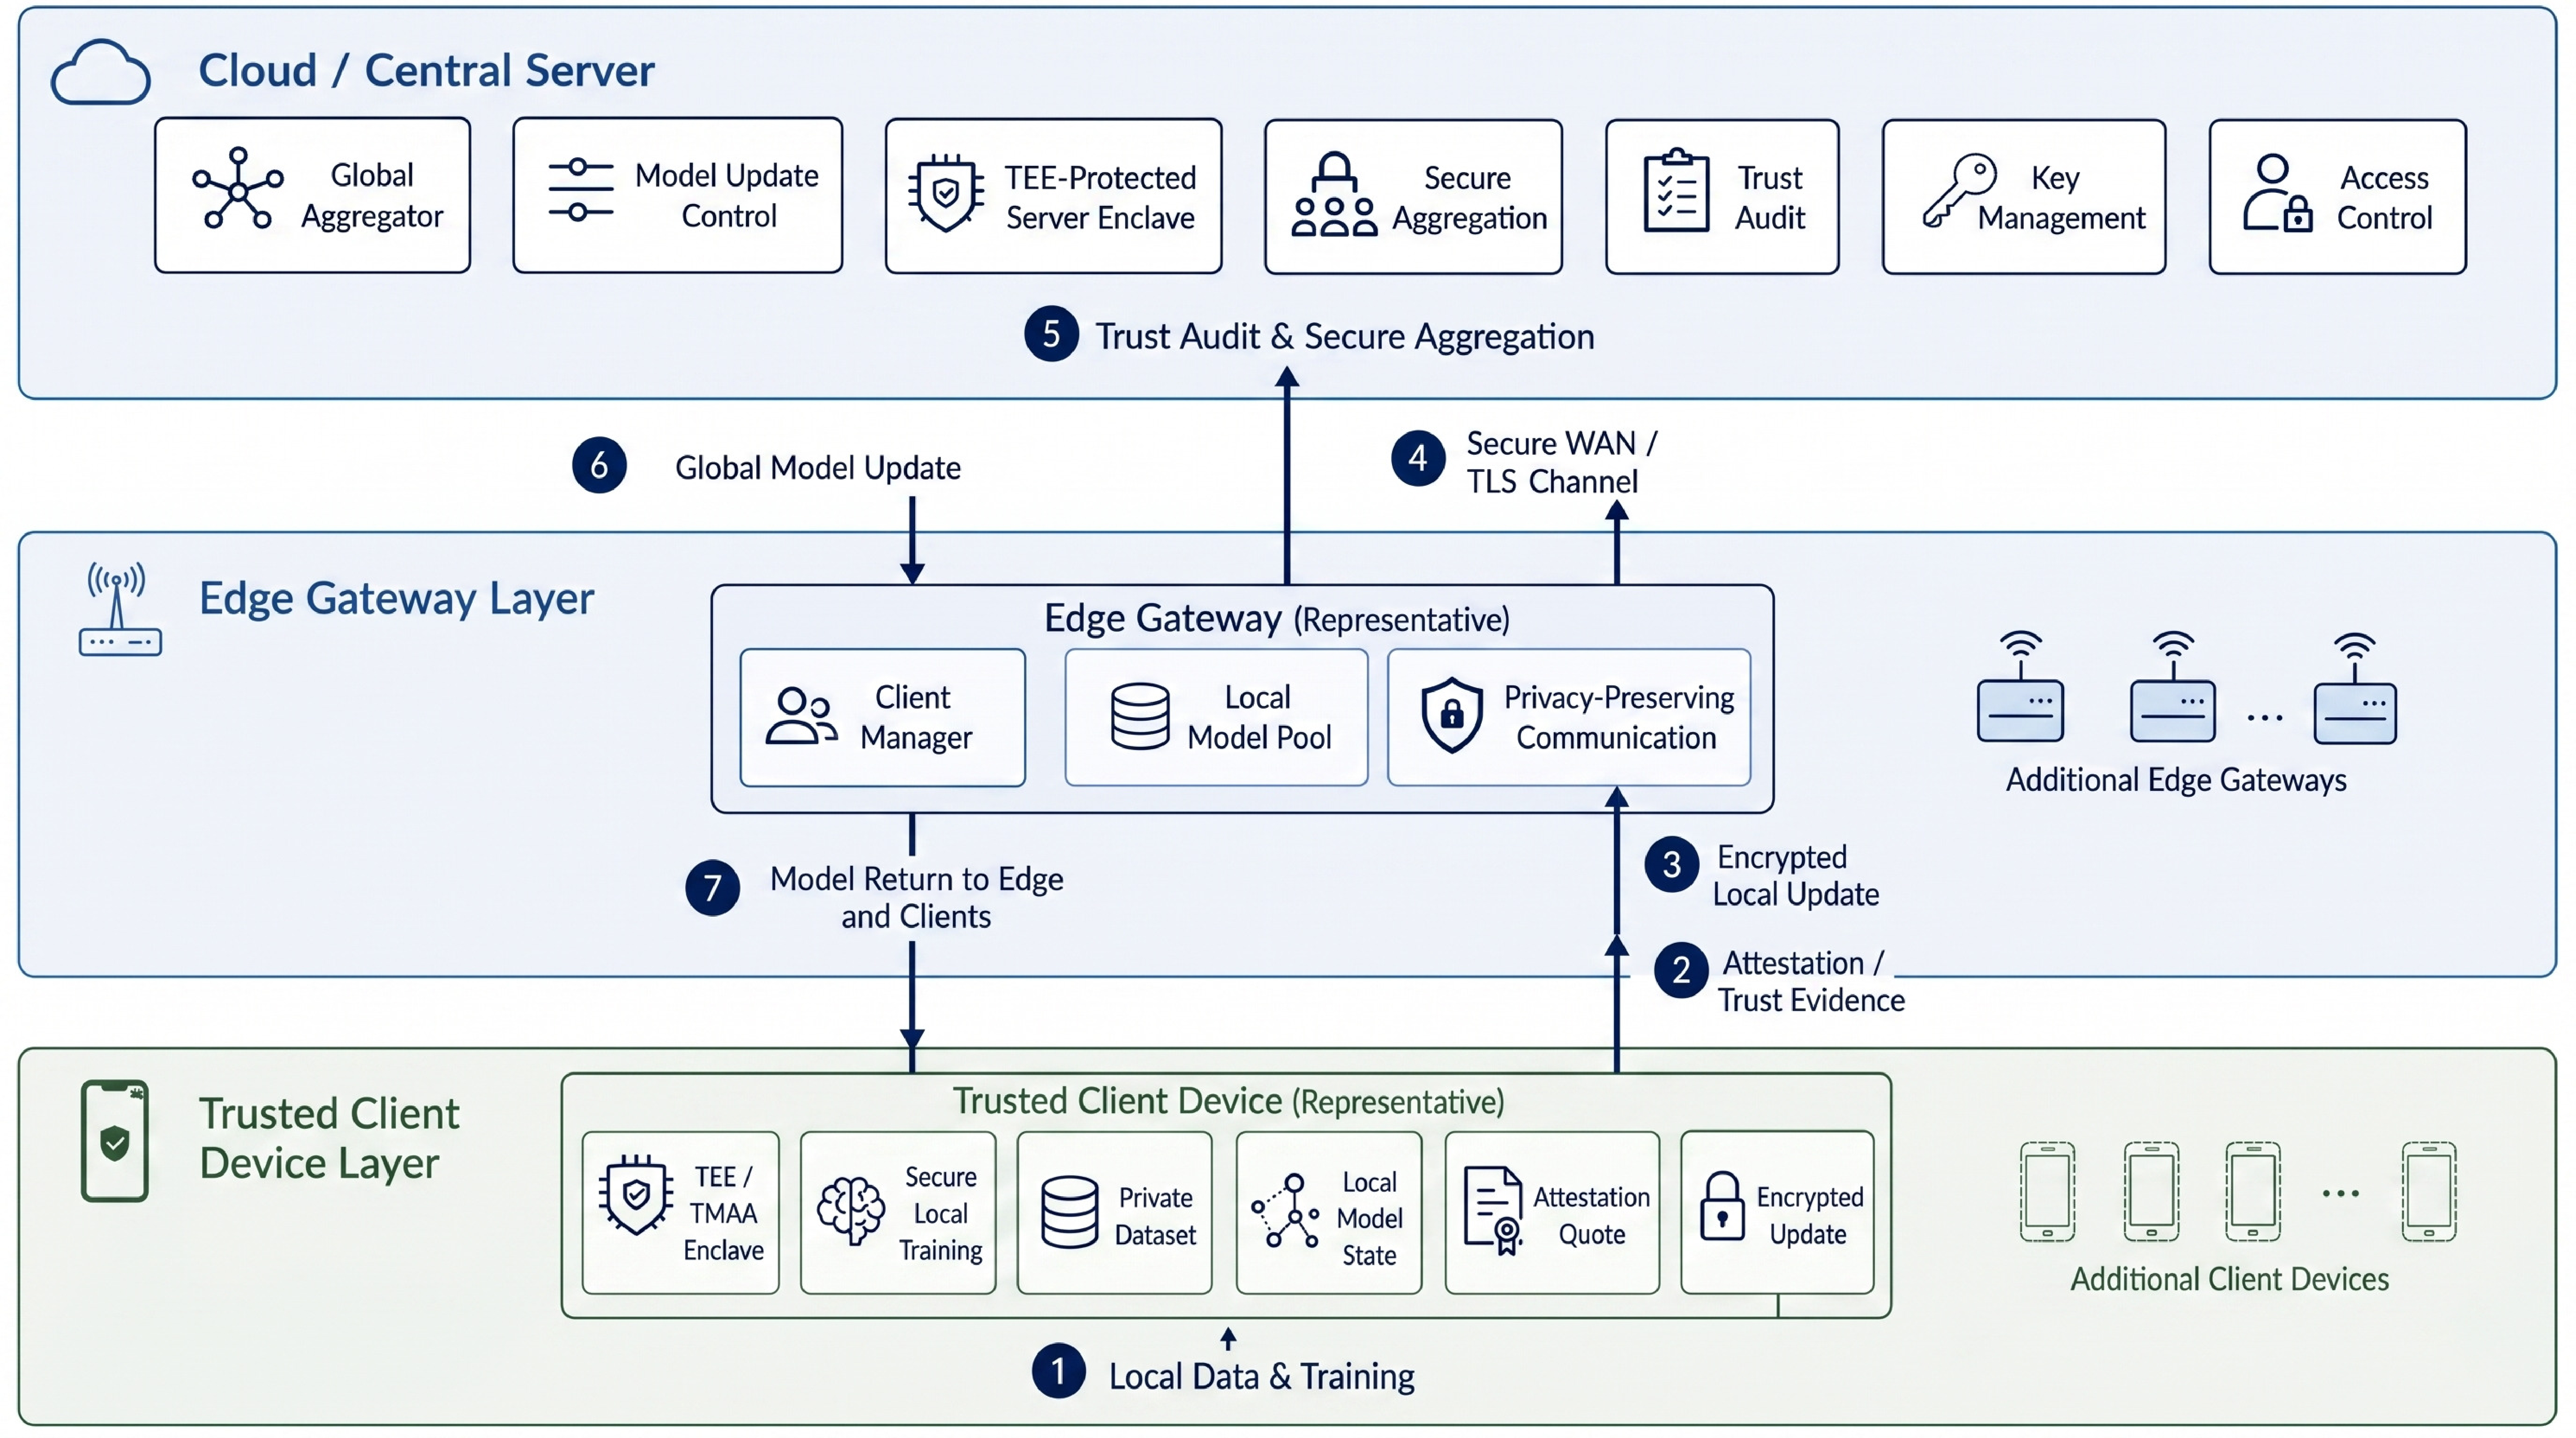
\includegraphics[width=0.84\textwidth]{fig1_system_arch.pdf}
    \caption{TEE-anchored client-edge-cloud architecture.}
    \label{fig:system_arch}
\end{figure}

\begin{figure}[t]
    \centering
    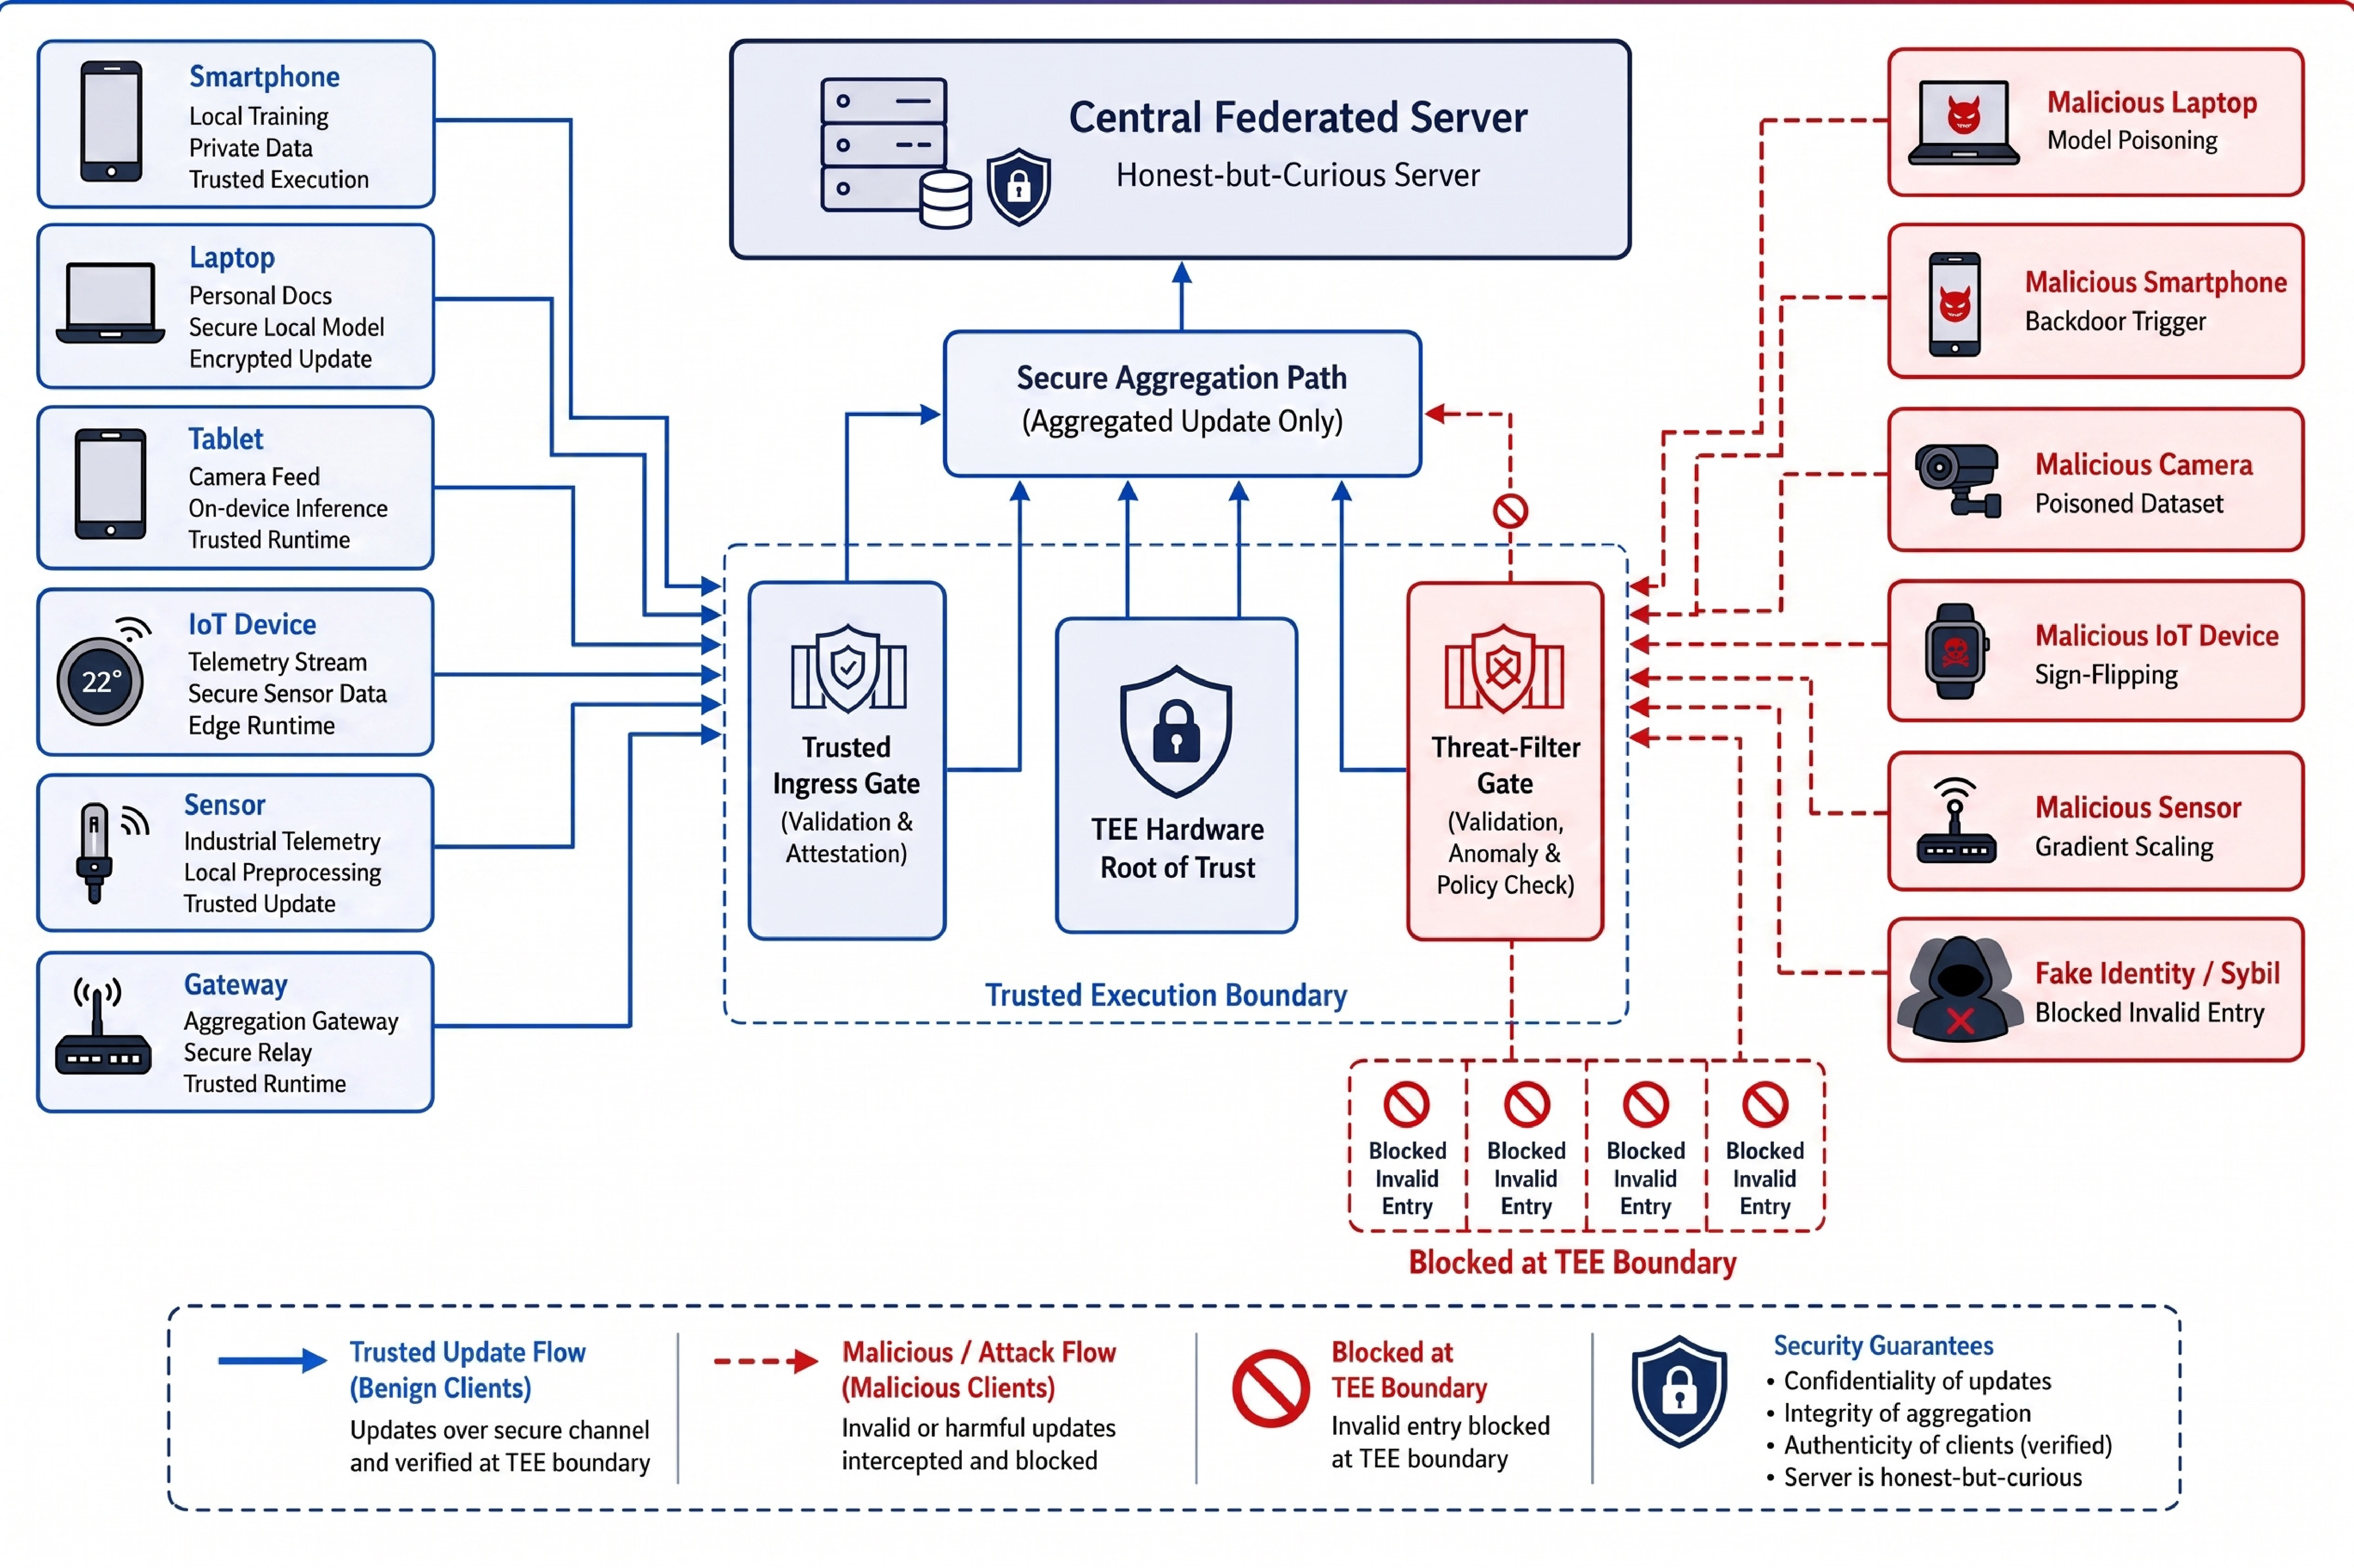
\includegraphics[width=0.80\textwidth]{fig2_threat_model.pdf}
    \caption{Composite poisoning and penetration threat model.}
    \label{fig:threat_model}
\end{figure}

\textbf{Threat model.} The server is honest-but-curious and follows the aggregation protocol; it sees individual updates and audit statistics but is not allowed to alter the stated state-transition rules. An admitted client may control local labels, samples, or optimization objectives and may perform label flipping, trigger backdoors, clean-label poisoning, semantic backdoors, sign flipping, or gradient scaling. The trust boundary is explicit. The TEE protects the measured execution path, device keys, report integrity, report freshness, and update binding against a compromised host, but it does not certify labels, samples, optimization objectives, or semantic intent. Consequently, an attacker may execute a data or objective-level poisoning strategy inside an otherwise valid measured process. The privacy-aware verification layer checks selected declared statistics without exposing raw samples, and the cloud-side content and temporal audit handles model-level effects that execution integrity cannot decide. A failed report or update-binding check is rejected at admission; a valid report does not imply a benign update. Physical probing and advanced microarchitectural side channels are excluded. The analytical assumption is fewer than 50\% malicious admitted clients; the 50\% experiment is an out-of-assumption stress test, not a Byzantine threshold or a theoretical guarantee. The server-held clean proxy set is a reference initializer for the content audit, while the trusted-peer branch supplies the corresponding operation when a server proxy is unavailable.

\textbf{Design goals.} Trust Flow aims to maintain convergence under the stated attacks, limit permanent false bans of long-tail clients, and preserve a clear assurance boundary. Execution evidence, privacy-aware statistical evidence, current content evidence, historical utility, and current risk retain separate meanings until layer-wise aggregation. The appended TrustReport is about 15 KB, server aggregation plus audit increases from 2.10 s to 4.85 s, the auxiliary secure path measures approximately 11 ms per admitted-client round for enclave transitions, memory pressure, and cryptographic aggregation, and device-side TEE Quote generation, signing, and lightweight monitoring are measured separately at approximately 12--15 ms per admitted-client round. The reported overhead is partitioned by system boundary so that communication, attestation, privacy-aware verification, and cloud audit costs are not conflated.

\section{Trust-Flow Framework}

Trust Flow divides each FL round into four linked stages: admission and runtime trust assessment, reference-based content auditing, dual-stream state evolution, and risk-gated layered aggregation. Figure~\ref{fig:framework} shows the full defense loop.

\begin{figure}[t]
    \centering
    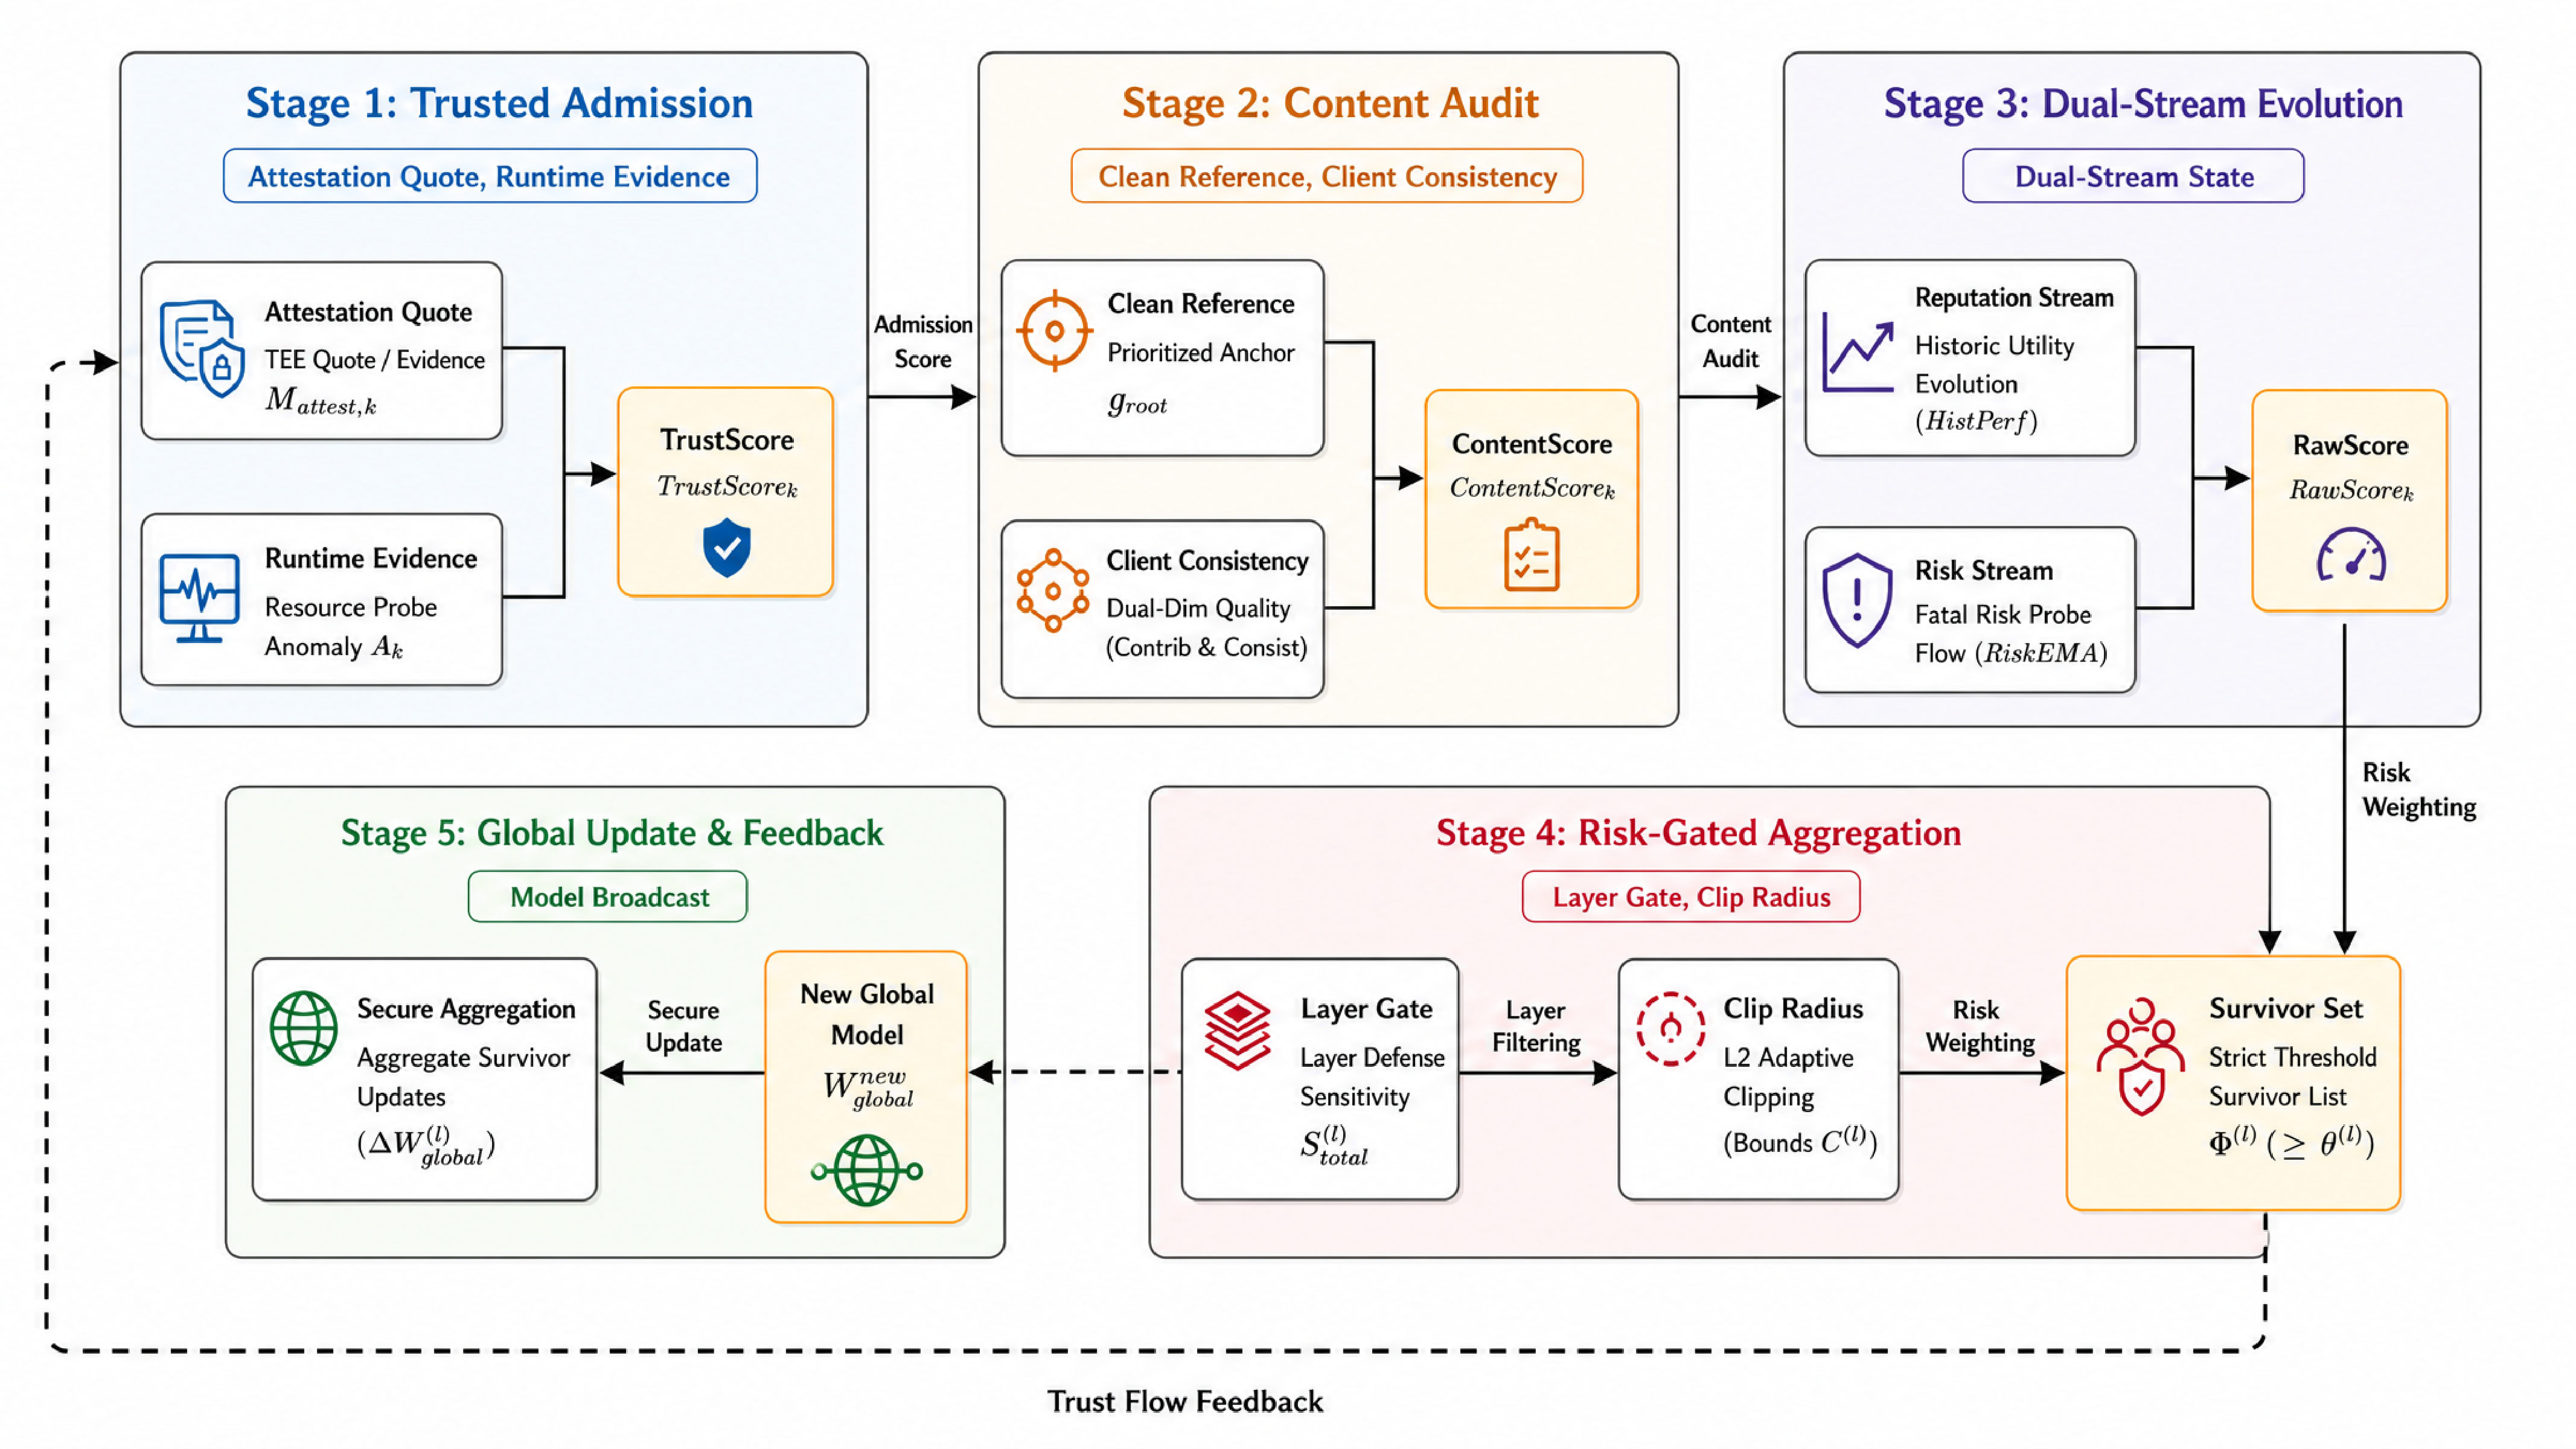
\includegraphics[width=0.86\textwidth]{fig3_arch.pdf}
    \caption{Overview of the four-stage trust-flow defense loop.}
    \label{fig:framework}
\end{figure}

The four stages output $TrustScore$, $ContentScore$, the slow $HistPerf$/fast $RiskEMA$ states, and finally $RawScore$. Invalid proofs are rejected first; privacy-aware statistics and current updates are then audited, temporal state is updated, and layer privileges are assigned. The same ordering applies during cold start: a new client receives a provisional first-round privilege, current evidence can reduce that privilege, and irreversible state transitions require accumulated evidence. A low one-round content score therefore remains recoverable for a Non-IID client, whereas persistent or current strong risk can restrict the corresponding update.

\subsection{Admission and Content Auditing}

Each admitted client must pass a TEE admission check. Let $M_{\text{attest},k}\in\{0,1\}$ denote whether the attestation report, its freshness nonce, and its binding to the round and update digest are valid. During initialization, the client invokes a device-unique key and generates a remote attestation quote containing a vendor-specific measurement digest, code identity, runtime configuration, round nonce, update digest, and monotonic freshness counter. Only clients passing this check receive communication privileges. During local training, the trusted management agent monitors standardized behavioral sequences
$\mathcal{X}_k=\{\Delta\text{grad},\Delta\text{loss},\text{instr\_dist}\}$. Let $h_k^{(t)}=H(\mathcal{X}_k^{(t)})/H_{\max}\in[0,1]$ be the normalized entropy after concatenating the three standardized feature histograms, where $H_{\max}$ is the entropy of their uniform concatenation. We use
\begin{equation}
    R_k^{(t)}=\exp(\lambda h_k^{(t)}),\qquad
    Z_k^{(t)}=\operatorname{clip}\!\left(w_aM_{\text{attest},k}+(1-w_a)(1-h_k^{(t)}),0,1\right),
\end{equation}
where $w_a=0.7$ and $\lambda=1.0$. High entropy is therefore treated as uncertain evidence, not as a direct maliciousness label.

Following a scalar Kalman filtering view, the trust estimate is updated as
\begin{equation}
    T_{k}^{-,(t)}=T_k^{(t-1)},\quad P_{k}^{-,(t)}=P_k^{(t-1)}+Q,
\end{equation}
\begin{equation}
\begin{aligned}
    K_k^{(t)}&=\frac{P_k^{-,(t)}}{P_k^{-,(t)}+R_k^{(t)}},\\
    T_k^{(t)}&=T_k^{-,(t)}+K_k^{(t)}(Z_k^{(t)}-T_k^{-,(t)}),\\
    P_k^{(t)}&=(1-K_k^{(t)})P_k^{-,(t)}.
\end{aligned}
\end{equation}
The observation $Z_k^{(t)}\in[0,1]$ is defined above; $Q=0.01$ is the fixed process-noise variance and $R_k^{(t)}$ is the entropy-derived observation variance. We initialize a fresh admitted client with $T_k^{(0)}=1$, $P_k^{(0)}=0.25$, $RiskEMA_k^{(0)}=0$, and $M_{\text{attest},k}=1$. The resulting privilege factor is
\begin{equation}
    TrustScore_k^{(t)}=M_{\text{attest},k}\,\operatorname{clip}\!\left(\frac{T_k^{(t)}}{1+P_k^{(t)}},0,1\right).
\end{equation}
High entropy increases $R_k^{(t)}$ and reduces the Kalman gain, so an uncertain observation cannot abruptly rewrite cross-round trust.

    The server then constructs a clean guiding direction. If a small clean validation gradient is available, $g_{root}=g_{root\_clean}$; otherwise, it uses admitted clients with high trust and low previous risk, with reference weights $\omega_k^{ref}=TrustScore_k^{(t)}(1-RiskEMA_k^{(t-1)})^2$. In the reported experiments, a balanced 500-sample proxy set (50 images per CIFAR-10 class) is held by the server and is not included in client training. The fixed proxy partition is part of the common experiment protocol; methods with a reference channel use it for their defined reference operation, while methods without that channel retain their own aggregation rule under the same data, initialization, and communication budget. The proxy supplies a stable guiding seed for content auditing; peer consistency and temporal states continue to provide evidence after initialization. When no such set is available, the trusted-peer branch constructs the corresponding reference from admitted updates. For each update, content quality combines reference consistency and peer consistency:
\begin{align}
    S_{contrib,k}  & =\max(0,\alpha_1+\alpha_2\cos(\Delta W_k,g_{root})),                                  \\
    S_{consist,k}  & =\frac{\sum_{j\ne k}TrustScore_j\max(0,\alpha_1+\alpha_2\cos(\Delta W_k,\Delta W_j))}
    {\sum_{j\ne k}TrustScore_j+\varepsilon},                                                               \\
    ContentScore_k & =\frac{(1+\beta_{fusion}^2)S_{consist,k}S_{contrib,k}}
    {\beta_{fusion}^2S_{consist,k}+S_{contrib,k}+\varepsilon}.
\end{align}
With $\beta_{fusion}>1$, the harmonic fusion favors the clean direction but still requires peer plausibility, preventing either collusion or Non-IID reference deviation from dominating alone.

\subsection{Dual-Stream State Evolution}

Single reputation scores confuse low utility caused by data skew with high risk caused by attacks. Trust Flow therefore separates client state into a historical utility stream and a short-term risk stream. Let $q_k^{(t)}=\operatorname{clip}(ContentScore_k^{(t)},0,1)$. The historical stream uses an explicitly decayed Beta model:
\begin{equation}
    a_k^{(t)}=\beta_h a_k^{(t-1)}+q_k^{(t)},\quad
    b_k^{(t)}=\beta_h b_k^{(t-1)}+1-q_k^{(t)},\quad
    HistPerf_k^{(t)}=\frac{a_k^{(t)}}{a_k^{(t)}+b_k^{(t)}+\varepsilon}.
\end{equation}
For a fresh client, $a_k^{(0)}=b_k^{(0)}=1$, hence $HistPerf_k^{(0)}=0.5$ rather than an unjustified perfect reputation. The decay factor is $\beta_h\in(0,1)$ and is fixed before test rounds. During the first round, a validly admitted client remains in NORMAL and can only receive a provisional privilege determined by current content and risk. The first-round evidence is recorded for the next state update; it cannot by itself trigger an irreversible blacklist. This policy gives the server an immediate control response through provisional weighting while reserving permanent decisions for cross-round evidence.

The history channel is intentionally slow, so low utility reduces privilege without immediate removal. The risk channel is fast: $RiskEMA_k^{(t)}=\beta_rRiskEMA_k^{(t-1)}+(1-\beta_r)Risk_k^{inst}$, where $Risk_k^{inst}$ is the maximum current probe. Thus benign history cannot average away a strong warning.

    Let $u_k^{(t)}=1-HistPerf_k^{(t)}$ and $r_k^{(t)}=RiskEMA_k^{(t)}$. The reported thresholds $(\tau_h,\tau_s,\tau_q,\tau_b)=(0.26,0.64,0.80,0.90)$ govern utility deficit, soft risk, quarantine, and blacklisting. A NORMAL client enters SUSPECT after two consecutive rounds with $u_k^{(t)}>\tau_h$ or $r_k^{(t)}\geq\tau_s$. A SUSPECT client enters QUARANTINE after three such consecutive rounds or one current-round probe with $Risk_k^{inst}\geq\tau_q$. A QUARANTINE client enters BLACKLIST after four consecutive rounds with $r_k^{(t)}\geq\tau_b$. Recovery from SUSPECT or QUARANTINE requires two consecutive rounds with $u_k^{(t)}\leq\tau_h$ and $r_k^{(t)}<\tau_s$; a BLACKLIST state is irreversible within an experiment. These counters are reset when the corresponding condition is not met, and the state update is completed before layer aggregation. Thus, first-round control and permanent admission decisions have different semantics: the former limits the current contribution, while the latter requires persistent evidence.

The two streams meet only when computing aggregation privilege:
\begin{align}
    RawScore_k^{(t)} & = (TrustScore_k^{(t)})^\alpha(ContentScore_k^{(t)})^\beta
    (HistPerf_k^{(t)})^\gamma \nonumber                      \\
               & \quad \times (1-RiskEMA_k^{(t)})^p .
\end{align}
The state transition is evaluated after current probes and before aggregation. This timing lets current risk veto a sleeper burst despite high history, while a low-similarity benign client remains recoverable through the slow stream.

\begin{figure}[t]
    \centering
    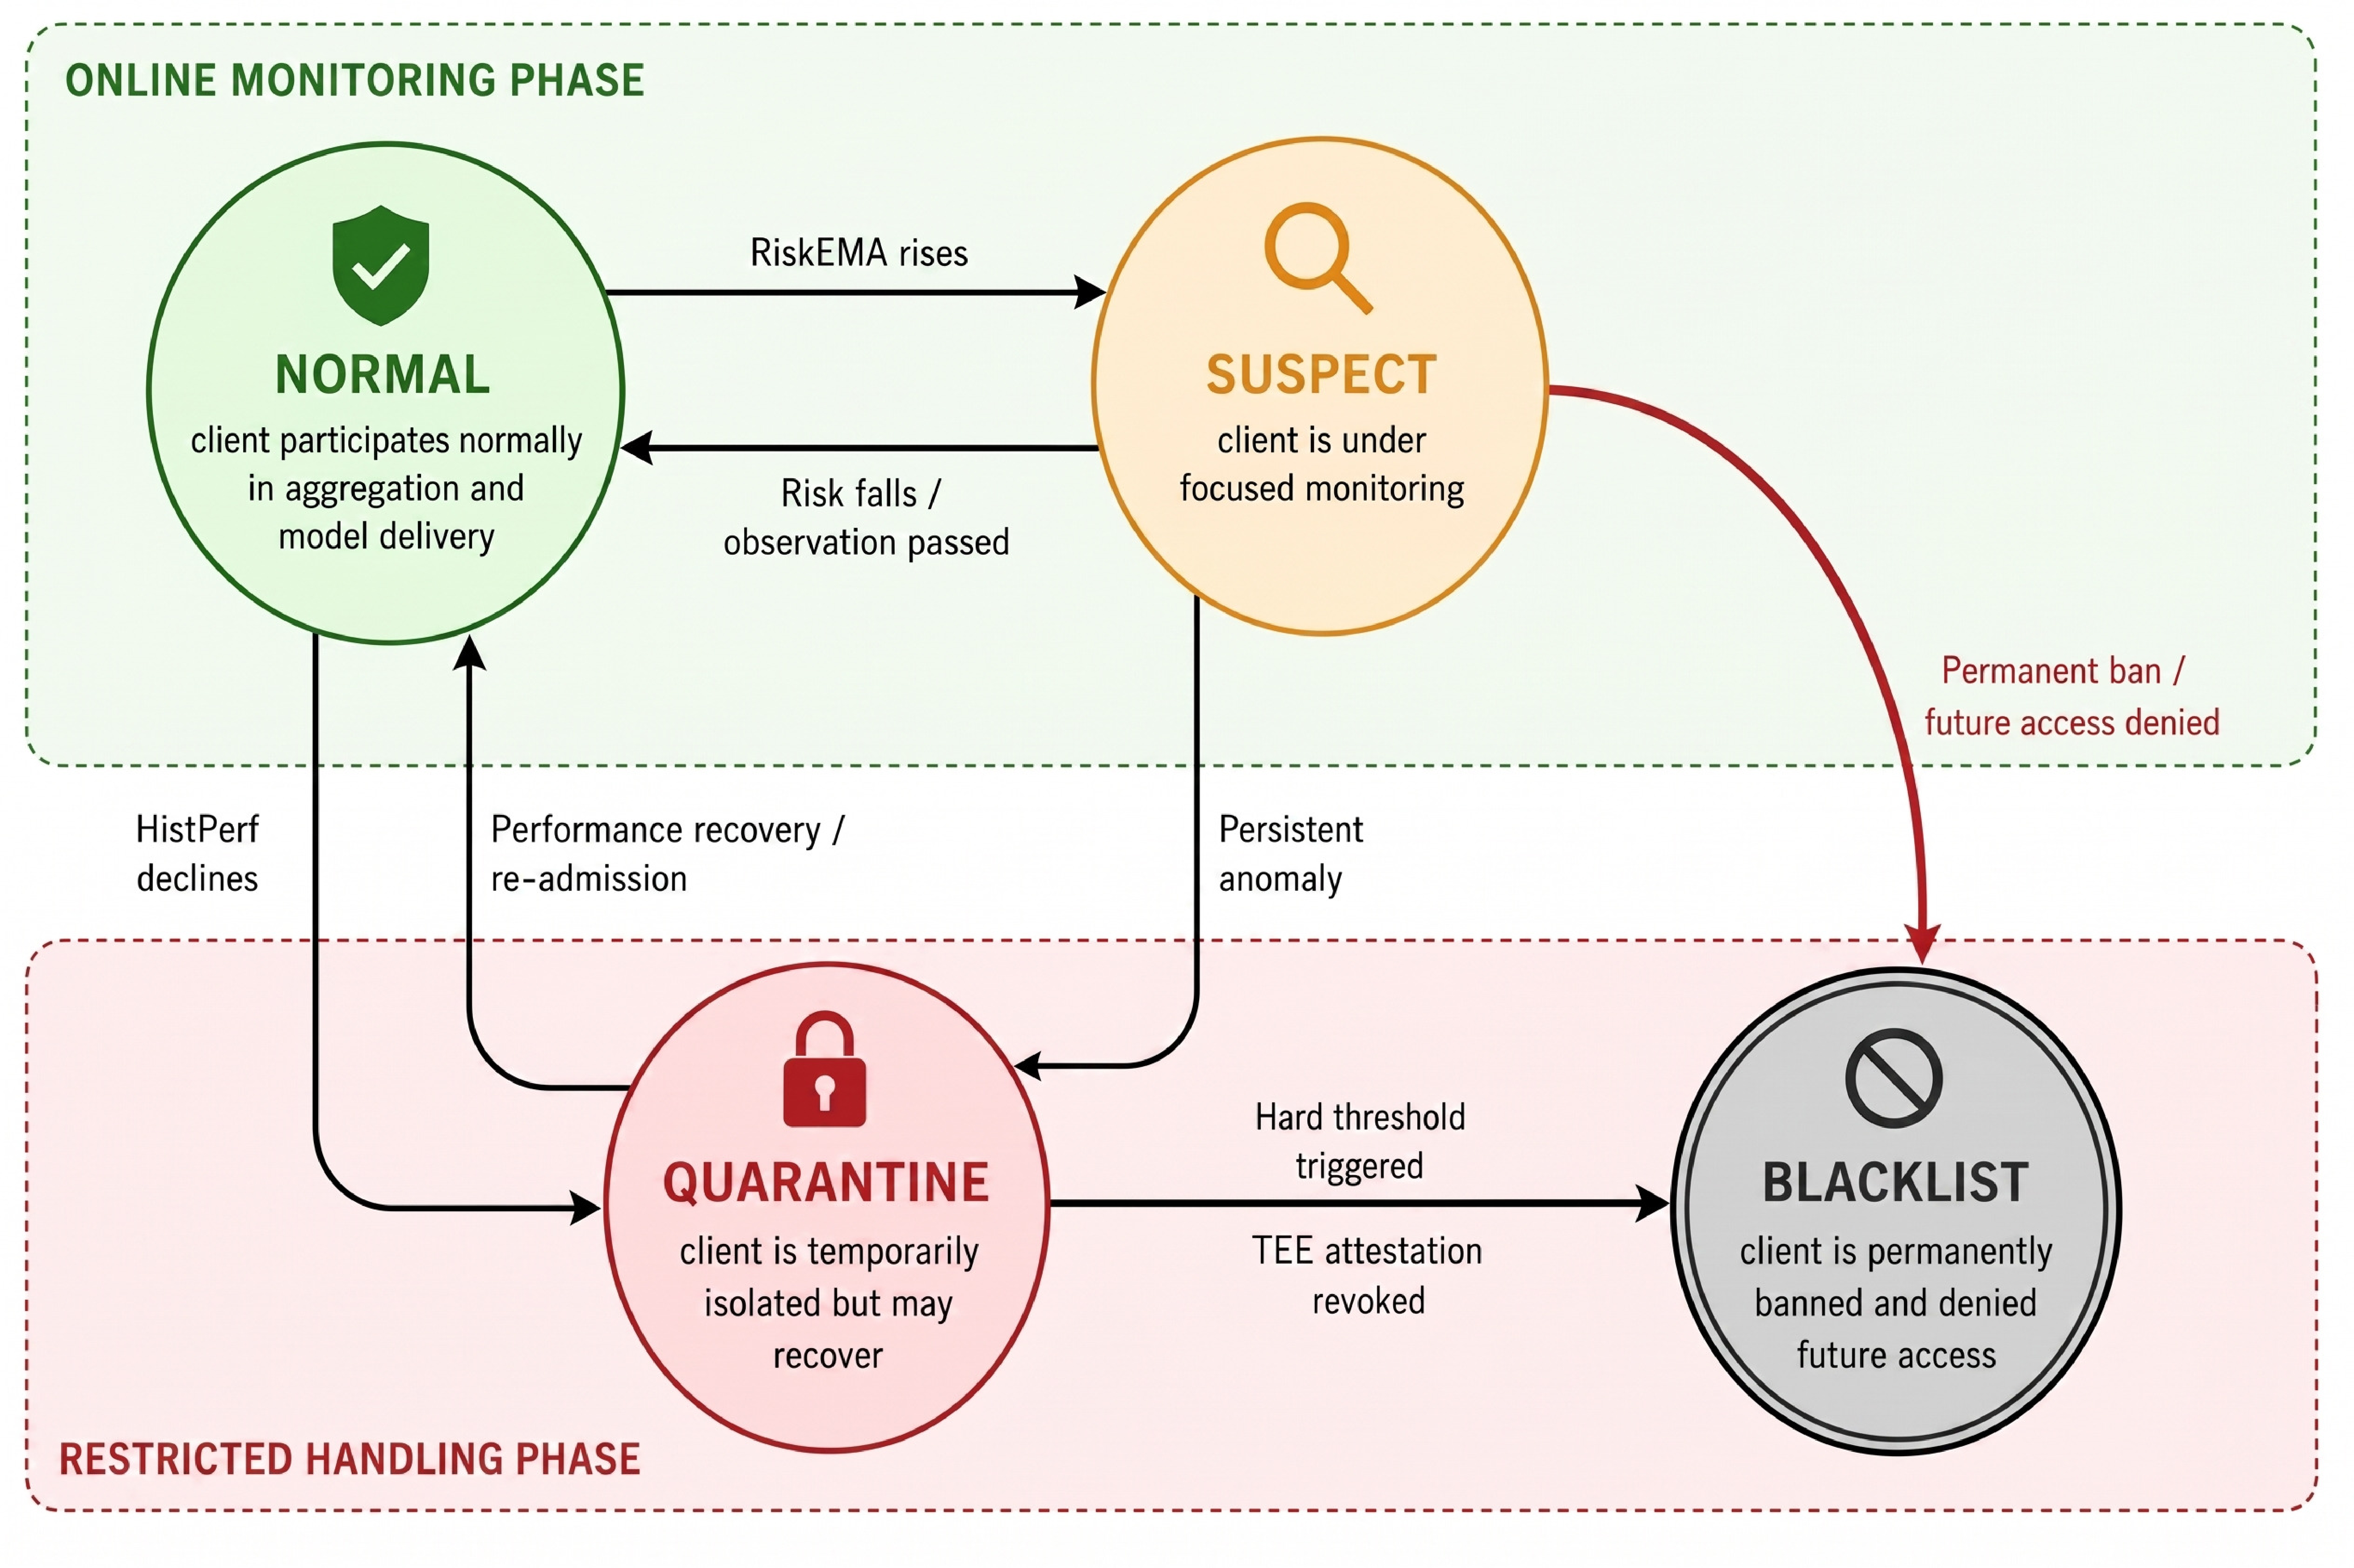
\includegraphics[width=0.76\textwidth]{fig4_state.pdf}
    \caption{Client state-transition automaton driven by historical utility and short-term risk.}
    \label{fig:state_machine}
\end{figure}

\subsection{Risk-Gated Layered Aggregation}

Backdoors often concentrate in deeper layers, whereas shallow feature layers may carry useful heterogeneous information. Trust Flow therefore assigns each layer $l$ a sensitivity score. With $L$ total layers, the three normalized components are
\begin{figure}[t]
    \centering
    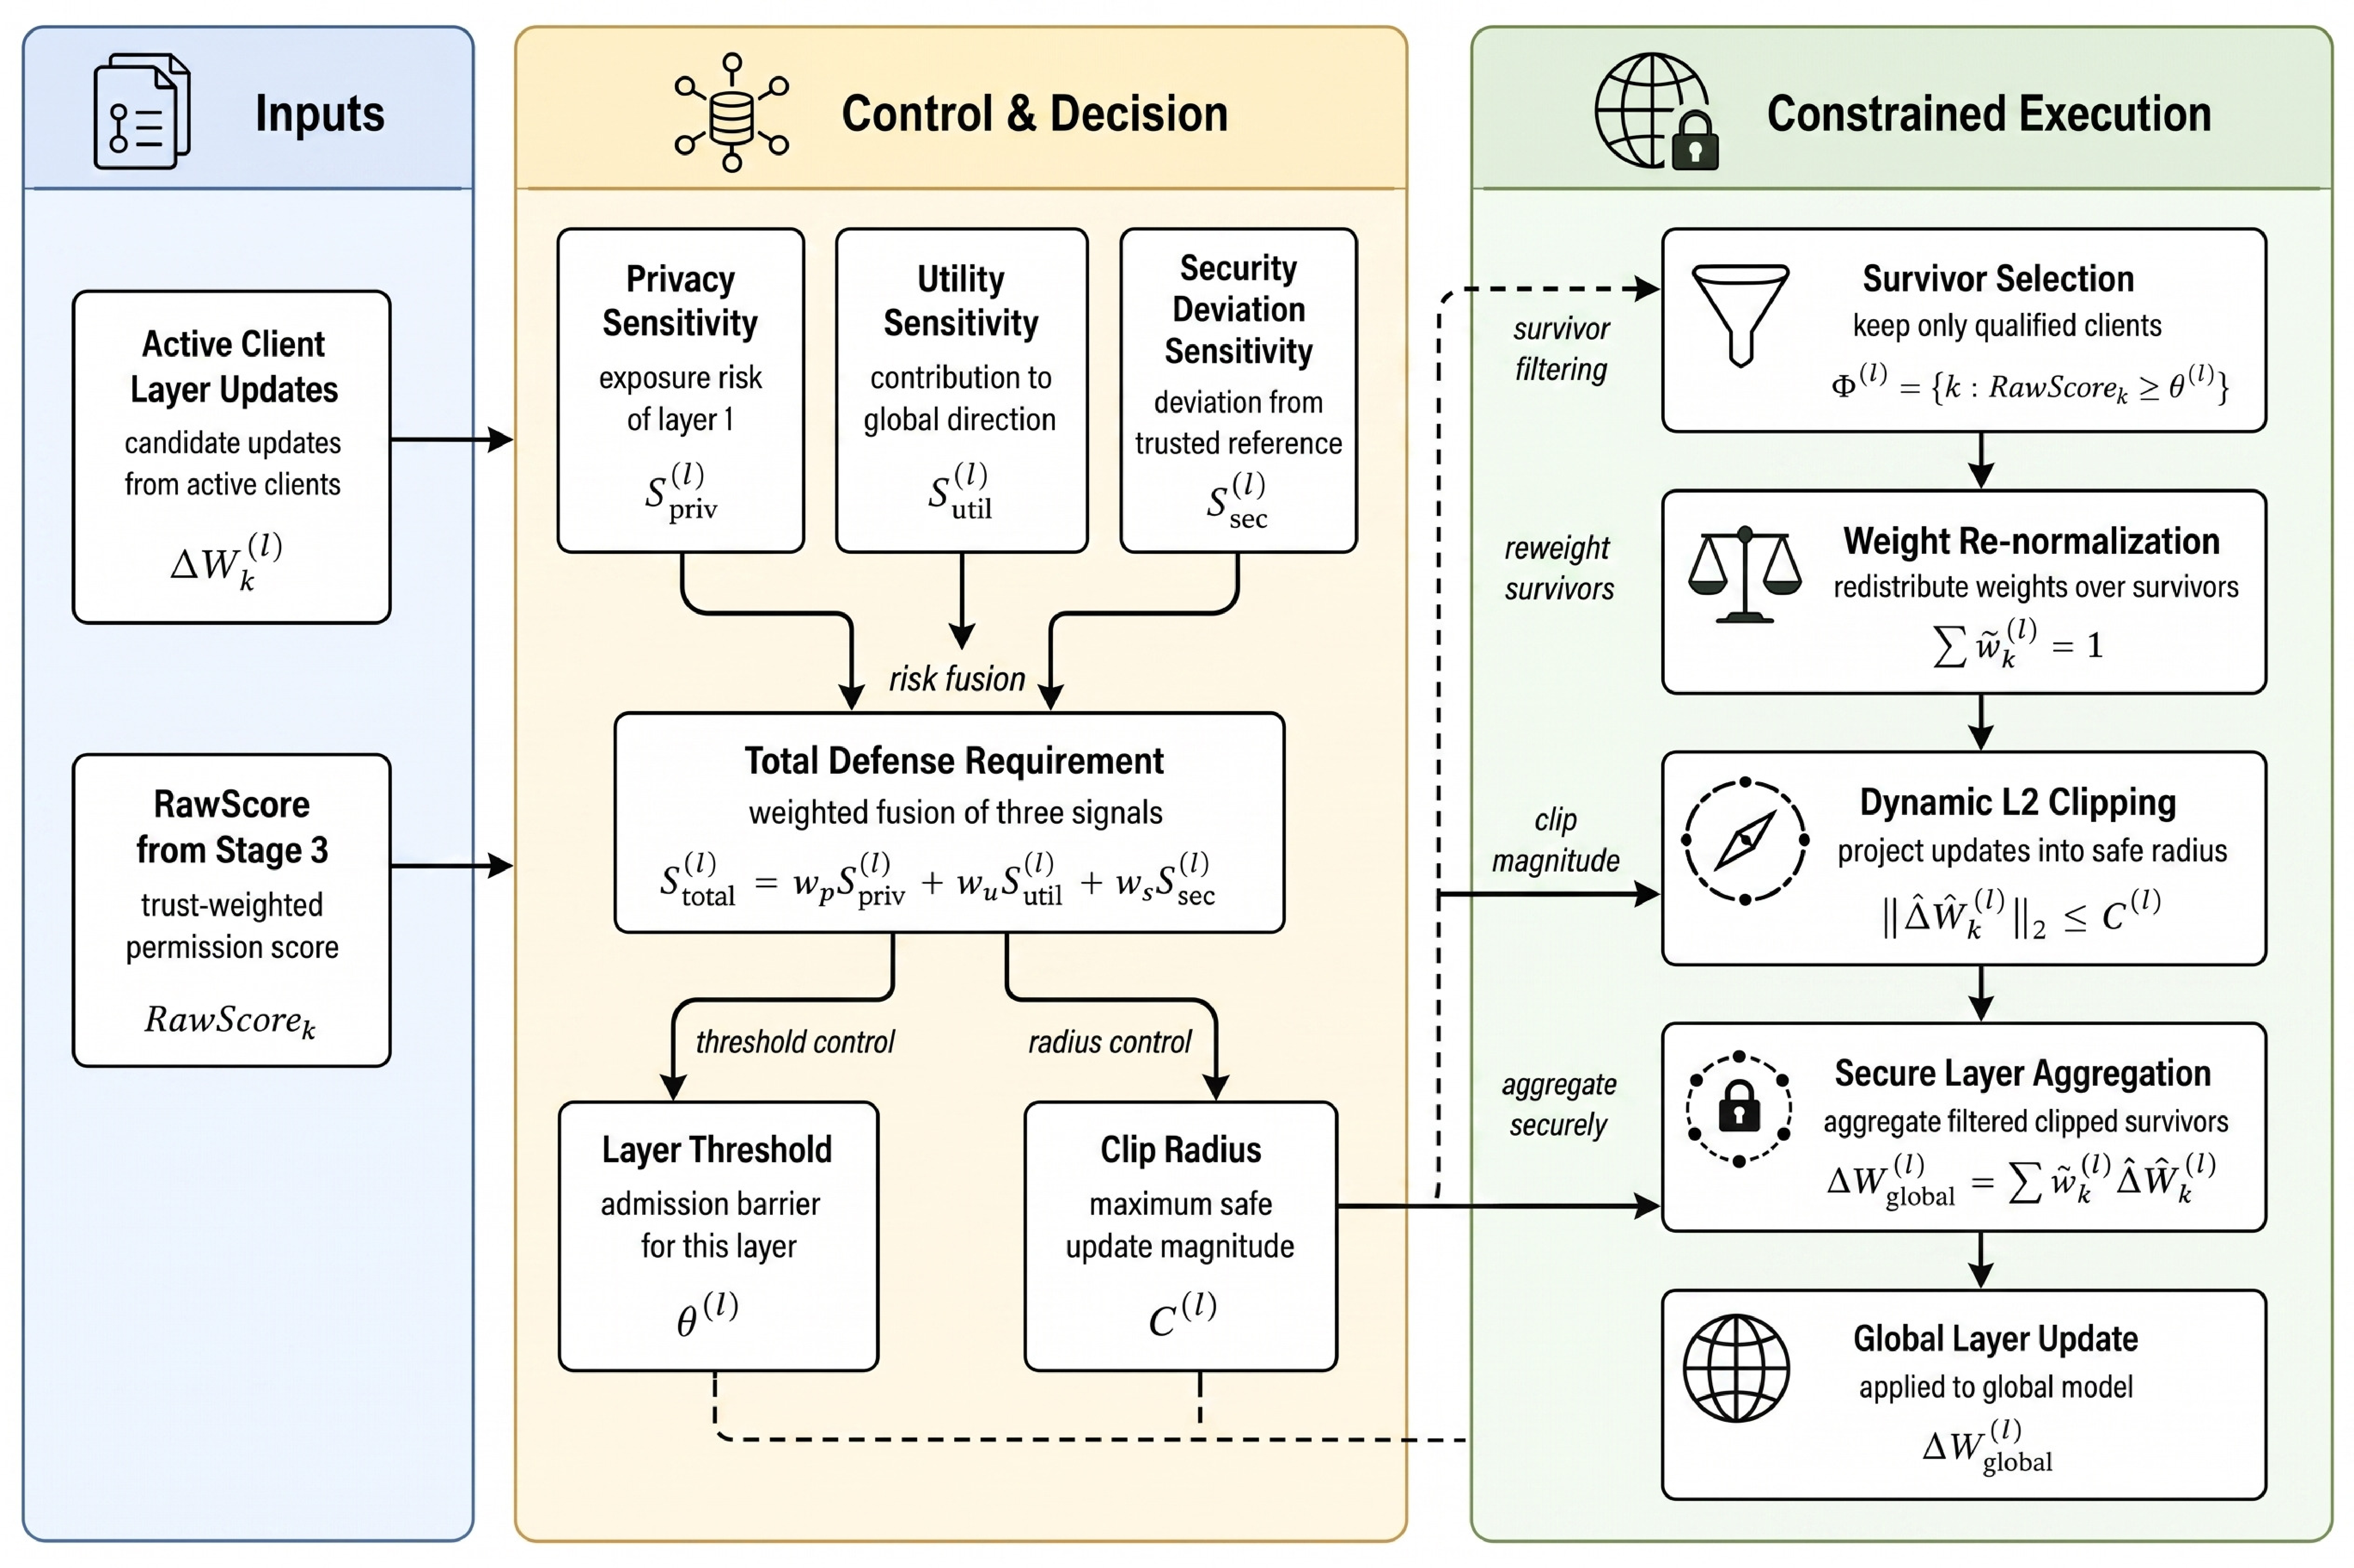
\includegraphics[width=0.78\textwidth]{fig5_layer.pdf}
    \caption{Risk-gated layer-wise clipping and differentiated aggregation.}
    \label{fig:layer_gating}
\end{figure}
\begin{equation}
\begin{aligned}
    S_{priv}^{(l)}&=\exp(-\tau_p l/L),\quad
    S_{util}^{(l)}=\frac{\|g_{root}^{(l)}\|_2}{\max_m\|g_{root}^{(m)}\|_2+\varepsilon},\\
    S_{sec}^{(l)}&=\frac{1}{2}\left(1-\frac{1}{|\mathcal{T}|}\sum_{k\in\mathcal{T}}
    \cos(\Delta W_k^{(l)},g_{root}^{(l)})\right).
\end{aligned}
\end{equation}
where $\mathcal{T}=\{k\in\mathcal{A}:M_{\text{attest},k}=1,\;RiskEMA_k^{(t-1)}<\tau_s\}$ is the trusted reference set. If this set is empty, the server uses the admitted set $\mathcal{A}$ only to normalize the layer score and records that no trusted peer reference was available. Hence $S_{priv}^{(l)},1-S_{util}^{(l)},S_{sec}^{(l)}\in[0,1]$. We use $S_{total}^{(l)}=w_pS_{priv}^{(l)}+w_u(1-S_{util}^{(l)})+w_sS_{sec}^{(l)}$, with $w_p,w_u,w_s=(0.3,0.3,0.4)$ and $w_p+w_u+w_s=1$, so $S_{total}^{(l)}\in[0,1]$. The threshold and clipping radius are
\begin{equation}
    \theta^{(l)}=\mu_{base}+\lambda_sS_{total}^{(l)},\qquad
    C^{(l)}=\frac{C_{base}}{S_{total}^{(l)}+\varepsilon_c}.
\end{equation}
Thus a layer with stronger suspicious drift becomes harder to enter and more tightly clipped; a layer that remains close to the reference keeps more capacity for benign heterogeneity.

We set $\tau_p=3.0$, $\varepsilon=\varepsilon_c=10^{-8}$, and define $C_{base}$ as the median trusted-client update norm before layer gating. These choices keep the sensitivity terms dimensionless and make the clipping scale robust to the round-wise update magnitude.

Survivors are $\Phi^{(l)}=\{k\in\mathcal{A}\mid RawScore_k^{(t)}\ge\theta^{(l)}\}$, and their weights are re-normalized:
\begin{equation}
    \tilde{w}_{k}^{(l)}=\frac{p_kRawScore_k^{(t)}}{\sum_{j\in\Phi^{(l)}}p_jRawScore_j^{(t)}+\varepsilon},\quad
    \widehat{\Delta W}_k^{(l)}=\frac{\Delta W_k^{(l)}}{\max(1,\|\Delta W_k^{(l)}\|_2/C^{(l)})}.
\end{equation}
The final update is $\Delta W_{global}^{(l)}=\sum_{k\in\Phi^{(l)}}\tilde{w}_{k}^{(l)}\widehat{\Delta W}_k^{(l)}$. Weight re-normalization prevents the removal of risky clients from shrinking the effective learning rate.

If $\Phi^{(l)}=\varnothing$ because a highly sensitive layer rejects all candidates, the server retains $k^*=\arg\max_{k\in\mathcal{A}}RawScore_k^{(t)}$ for that layer, assigns it unit normalized weight, and still applies the clipping radius $C^{(l)}$. This fallback keeps the layer update defined without weakening the threshold for the other clients.

This layer-wise control preserves useful shallow representations while hardening layers with stronger suspicious drift. A semantic backdoor that mainly shifts deep features can therefore be clipped or rejected in those layers without imposing the same threshold on benign shallow features. Re-normalization is coupled to this decision: after unsafe mass is removed, the surviving data-size-weighted scores are projected back to a valid aggregation simplex, avoiding an implicit learning-rate decay.

\subsection{Risk Probe Computation}

The short-term risk stream uses probes that are intentionally redundant rather than individually decisive. For update $k$ in round $t$, the normalized channels are
\begin{align}
 r_{grad,k}^{(t)}&=\operatorname{clip}\!\left(\frac{1-\cos(\Delta W_k,g_{root})}{2},0,1\right),\\
 r_{amp,k}^{(t)}&=\operatorname{clip}\!\left(\frac{\|\Delta W_k\|_2}{\operatorname{median}_j\|\Delta W_j\|_2+\varepsilon}-1,0,1\right),\\
 r_{clean,k}^{(t)}&=\operatorname{clip}\!\left(\frac{\mathcal{L}_{probe}(W+\Delta W_k)-\mathcal{L}_{probe}(W)}{\delta_{clean}+\varepsilon},0,1\right),\\
 r_{trigger,k}^{(t)}&=\operatorname{clip}\!\left(\frac{\mathrm{KL}(\mathcal{H}(A_{base})\|\mathcal{H}(A_k))}{\delta_{trigger}+\varepsilon},0,1\right),\\
 \bar c_k^{(t)}&=\frac{\sum_{j\ne k}TrustScore_j\,c_{kj}}{\sum_{j\ne k}TrustScore_j+\varepsilon},\quad
 r_{peer,k}^{(t)}=\operatorname{clip}(1-\bar c_k^{(t)},0,1),
\end{align}
where $c_{kj}=\cos(\Delta W_k,\Delta W_j)$. For the trigger probe, $A_{base}$ is the activation histogram of the current global model on the server-held proxy set and $A_k$ is the corresponding histogram after applying candidate update $k$. We use 32-bin histograms from the last convolutional block and the pre-classifier representation. In each round, $\delta_{clean}$ and $\delta_{trigger}$ are set to the median plus three median absolute deviations of the corresponding values over $\mathcal{T}$, making the calibration independent of the candidate under test. Define $Risk_k^{inst}=\max\{1-M_{\text{attest},k},r_{grad,k},r_{amp,k},r_{clean,k},r_{trigger,k},r_{peer,k}\}$.

The maximum preserves complementary warnings: gradient and amplitude channels expose parameter attacks, whereas clean-loss and activation channels target stealthier backdoors. Peer disagreement is supporting evidence because benign long-tail updates may disagree with the majority. The execution order is reference construction, current-update audit, state update, and layer aggregation.

\subsection{Assurance Composition and Reference Role}

The four evidence sources have complementary responsibilities. Attestation and privacy-aware verification establish whether the declared execution and selected statistics satisfy the admission policy. They do not certify the semantic intent of the local objective. The cloud audit examines the submitted update and its behavior on the available reference or peer evidence, and the temporal streams determine whether an isolated observation is transient or persistent. This composition prevents an execution-valid but semantically harmful update from being accepted solely because it is signed, while also preventing a single low-similarity observation from permanently removing a benign long-tail client.

The clean proxy is therefore a reference initializer and calibration source, rather than a replacement for the trust flow. It supplies a stable direction and a common probe interface when a small server-held set is available. The peer-reference branch preserves the same content and temporal decision sequence when the deployment supplies no proxy set. In either branch, the final decision is made from the update evidence, the state transitions, and the layer-wise aggregation rule; no single reference observation is treated as a maliciousness label.

\section{Experiments}

\subsection{Setup}

Experiments use Flower 1.5.0 and PyTorch on CIFAR-10 with a CIFAR-10-adapted ResNet-18: the first convolution uses a $3\times3$ kernel with stride one, the initial max-pooling layer is removed, and the classifier has ten outputs. Training and trusted execution are performed in two real hardware configurations based on Intel and AMD TEE-capable processors. NVIDIA A10 GPUs execute model training, whereas the CPU-side TEEs isolate attestation, trusted monitoring, report generation, and admission-state processing. Both hardware configurations execute the same request/response procedure, nonce-based freshness verification, measured-code identity checking, round and update-digest binding, protected report generation, and admission decision. The testbed uses anonymized servers with Intel and AMD dual-CPU configurations and five NVIDIA A10 GPUs; the software stack is Ubuntu 20.04.6 LTS and CUDA 12.8. The 50,000 training images are partitioned into a shared 5,000-image client pool, replicated as a common base subset for all clients, and 45,000 exclusive images: clients 0--9 use an IID split, clients 10--14 use Dirichlet $\alpha=1.0$, and clients 15--19 use Dirichlet $\alpha=0.1$. Separately, the server holds a balanced 500-image proxy set (50 per class) from the held-out CIFAR-10 reference partition; it is disjoint from client training and final evaluation. The fixed proxy partition and initialization are shared across all methods; reference-dependent methods use it for their defined guiding operation and probes, while methods without a reference channel retain their standard aggregation rule. All methods use the same optimizer, communication budget, client partition, and initial model. Five independent seeds are run on each hardware configuration; means and standard deviations are computed over the resulting ten platform-seed runs.

The formal 30\% attack setting uses six malicious clients: Client 0 performs untargeted label flipping with $\gamma=0.5$; Client 1 injects a fixed $3\times3$ lower-right trigger into 20\% of local samples and targets class 0; Client 2 uses label-preserving clean-label perturbations on 20\% of local samples with the same target; Client 3 applies a fixed semantic attribute bias to 20\% of local samples, with the biased subset assigned to class 0; Client 4 applies untargeted sign flipping; and Client 5 applies untargeted gradient scaling by a factor of 100. Clients 1--3 are evaluated as targeted attacks, whereas Clients 0, 4, and 5 are evaluated through clean loss, convergence, and detection state. Attack behaviors are active in every local training round; no attack is introduced only after observing the global trajectory. Five Sybil nodes without valid certificates and three free-rider nodes with forged low workload are used only to validate Phase-One gating. These eight nodes are intercepted before statistical aggregation, so later metrics are computed over the 20 admitted clients. Malicious updates that pass hardware attestation represent an attacker operating inside an admissible training process; post-attestation host tampering is excluded by the stated threat model. Each run uses 30 rounds and three local epochs. Aggregate values are averaged over the pooled platform-seed runs; state trajectories use one fixed seed per platform.

    Clean accuracy and targeted ASR are reported as mean and standard deviation over the ten platform-seed runs. For each targeted behavior $a\in\{\mathrm{trigger},\mathrm{clean},\mathrm{semantic}\}$, let $\mathcal{B}_a$ be its trigger- or attribute-bearing test subset and $y_a^*$ its declared target. We define $ASR_a=|\{x\in\mathcal{B}_a:\arg\max f(x)=y_a^*\}|/|\mathcal{B}_a|$ and report the macro-average $ASR_{target}=\frac{1}{3}\sum_a ASR_a$. The three attack-specific quantities are retained separately in the convergence traces; the headline table uses the macro-average to avoid assigning a larger weight to any one targeted behavior. Untargeted label/sign/scaling behavior is not folded into this numerator and is assessed through clean accuracy, loss, and state-transition time. Permanent-ban FPR is computed only for benign clients that are irreversibly blacklisted, while temporary SUSPECT or QUARANTINE states are recoverable control actions. Stateless baselines have no equivalent permanent-ban state, so their FPR is reported as N/A rather than compared numerically. All methods share the same client partition, initial model, optimizer, communication budget, attack schedule, reference availability, and Non-IID split; each method uses the shared evidence according to its own defined decision rule.

\begin{table}[t]
    \centering
    \caption{Experimental configuration and main hyperparameters.}
    \label{tab:setup}
    \small
    \begin{tabular*}{\textwidth}{@{\extracolsep{\fill}} p{2.45cm} p{5.2cm} p{4.25cm}}
        \toprule
        Category & Setting & Value \\
        \midrule
        FL task & Dataset/model/admitted clients & CIFAR-10/CIFAR-adapted ResNet-18/$K=20$ \\
        Optimization & Local epochs, lr, momentum, rounds & $3$, $0.001$, $0.9$, $30$ \\
        Data heterogeneity & Shared client pool; server proxy; Group A/B/C & $5000$; $500$; $\alpha=1.0,0.1$ \\
        Trust streams & $\alpha_1,\alpha_2,\beta_{fusion}$; $\beta_h,\beta_r$ & $0.6,0.4,2.0$; $0.9,0.85$ \\
        Admission filter & $w_a,\lambda,Q$; $T_0,P_0,RiskEMA_0$ & $0.7,1.0,0.01$; $1,0.25,0$ \\
        Layer gating & $\alpha,\beta,\gamma,p$; $\mu_{base},\lambda_s$ & $3.0,1.0,0.5,1.0$; $0.4,1.2$ \\
        Sensitivity & $\tau_p; w_p,w_u,w_s$ & $3.0; 0.3,0.3,0.4$ \\
        Numerical stability & $\varepsilon,\varepsilon_c$; $C_{base}$ & $10^{-8},10^{-8}$; median trusted norm \\
        State machine & $\tau_h,\tau_s,\tau_q,\tau_b$; persistence & $0.26,0.64,0.80,0.90$; $2,3,4$ rounds \\
        \bottomrule
    \end{tabular*}
\end{table}

\subsection{Overall Defense Performance}

Figure~\ref{fig:main_results} summarizes convergence, the three attack-specific ASR traces, trust-state trajectories, and feature separation. Under the stated 30\% mixed-attack protocol, all six attack behaviors are active concurrently in every local round; this is a simultaneous-attack test rather than a collection of one-at-a-time trials. Trust Flow reaches 92.31\% clean accuracy and 10.21\% macro-averaged targeted ASR, close to the 10\% random-target rate for ten CIFAR-10 classes. Client-state tracing shows how the assurance layers cooperate: execution-valid clients remain eligible for semantic auditing, current probes expose harmful update behavior, and the temporal streams decide whether the observation is transient or persistent. A legitimate long-tail node may receive provisional restrictions without losing its accumulated history, whereas persistent risk can move the client through the defined state transitions. These observations describe the stated protocol and the evidence interfaces used by the compared methods.

Trajectories show sustained risk for label, trigger, semantic, sign, and scaling attacks, whereas a long-tail benign client can recover because its risk does not persist. The t-SNE view is used as a visualization of the resulting trust-state features; the quantitative claims are taken from the accuracy, ASR, and state-transition metrics.

\begin{figure}[t]
    \centering
    \begin{minipage}{0.49\textwidth}
        \centering
        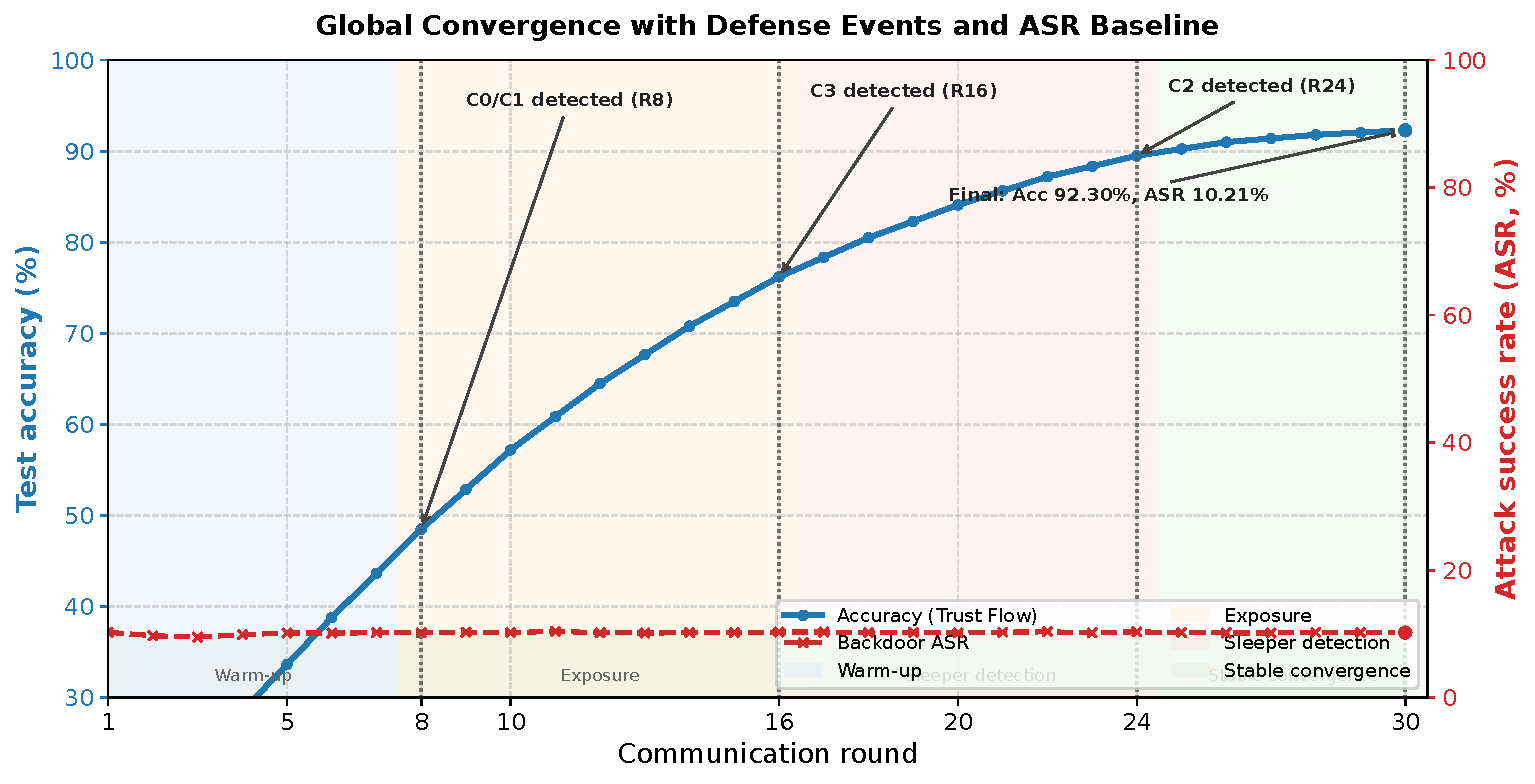
\includegraphics[width=\linewidth]{fig6_convergence_asr.pdf}
        \vspace{-3pt}
        {\scriptsize (a) Accuracy and ASR convergence.}
    \end{minipage}\hfill
    \begin{minipage}{0.49\textwidth}
        \centering
        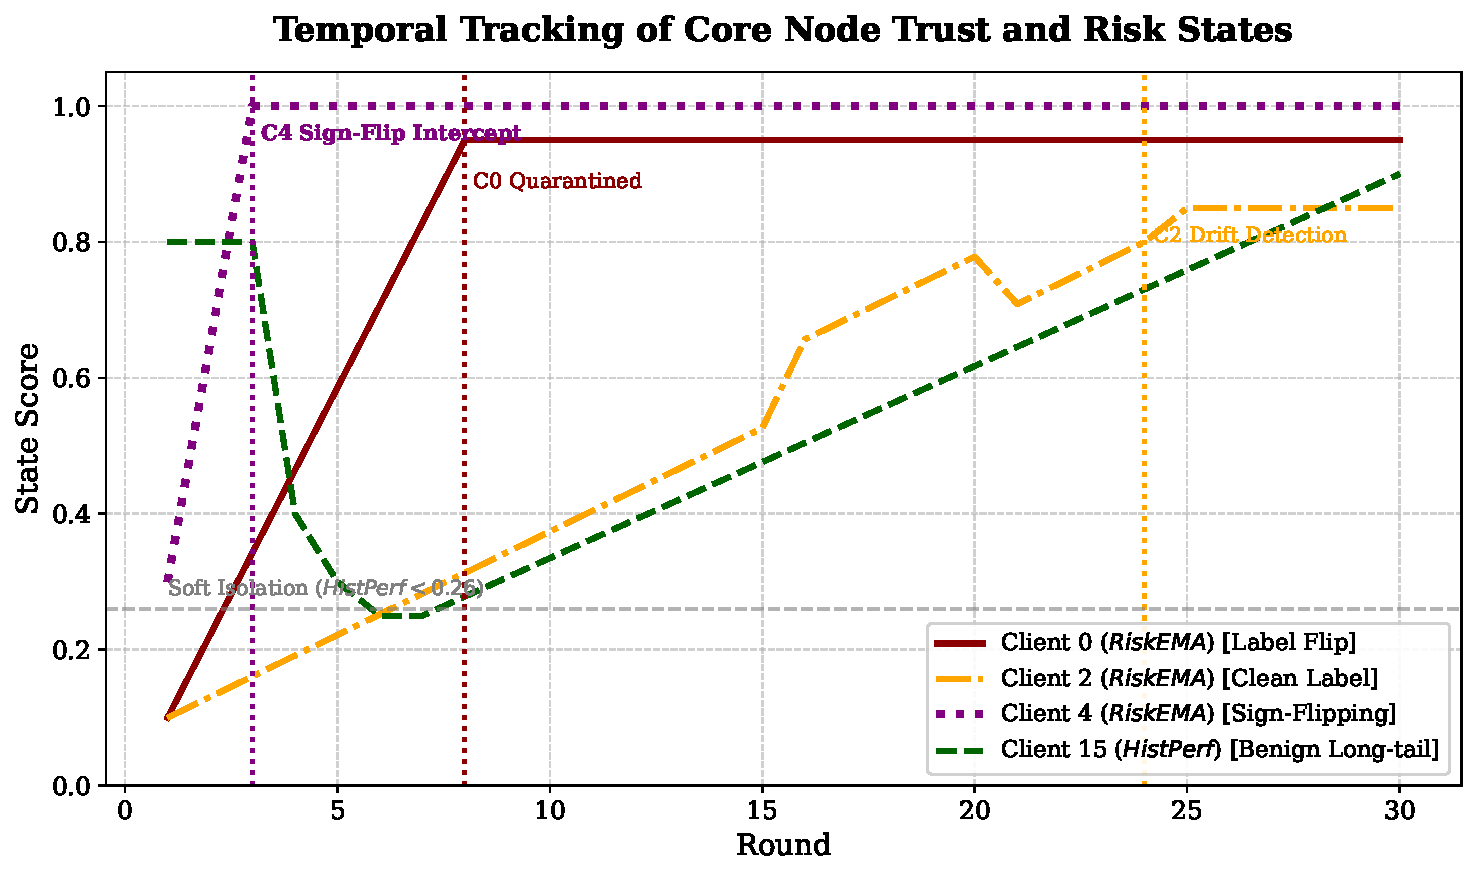
\includegraphics[width=\linewidth]{fig7_node_state_evolution.pdf}
        \vspace{-3pt}
        {\scriptsize (b) Node trust and risk trajectories.}
    \end{minipage}
    \par\vspace{16pt}
    \begin{minipage}{0.57\textwidth}
        \centering
        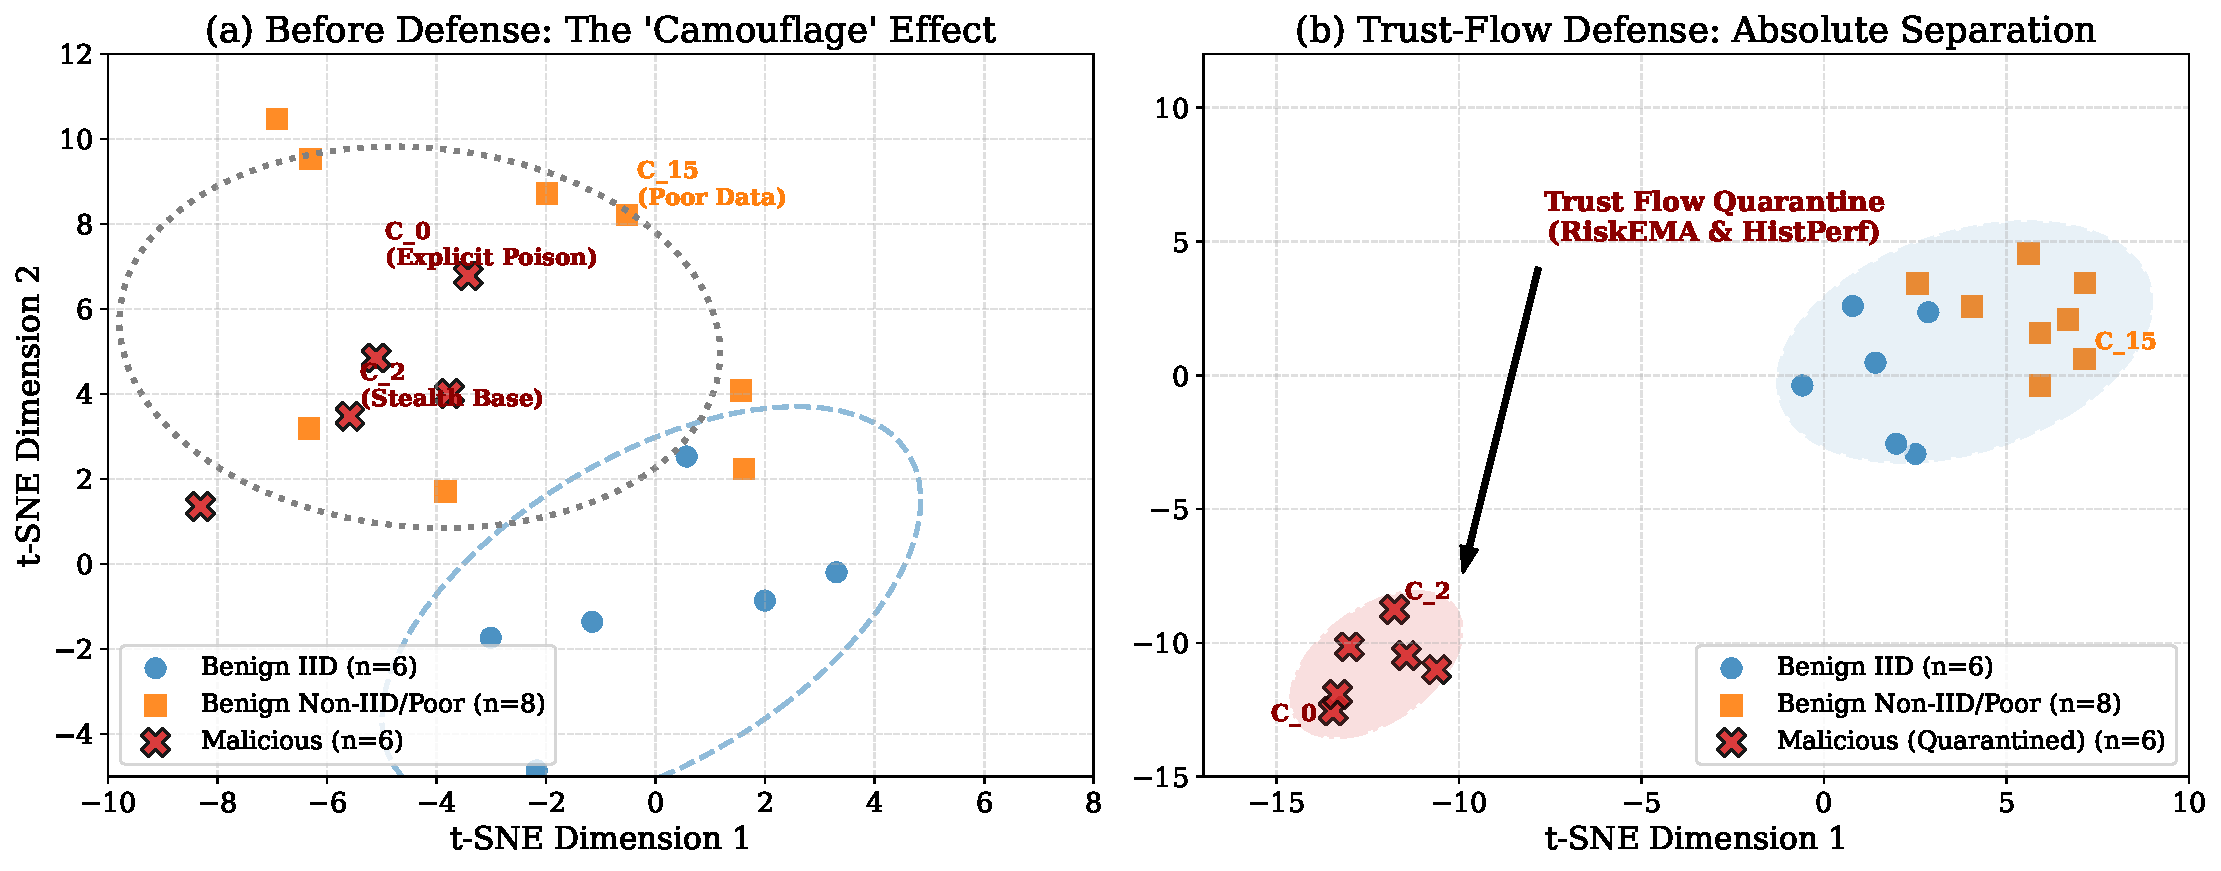
\includegraphics[width=\linewidth]{fig8_tsne_visualization.pdf}
        \vspace{-3pt}
        {\scriptsize (c) t-SNE separation before/after defense.}
    \end{minipage}
    \caption{Main defense behavior under mixed attacks.}
    \label{fig:main_results}
\end{figure}

\begin{table}[t]
    \centering
    \begin{threeparttable}
        \caption{Performance comparison under 30\% mixed attacks and boundary stress testing.}
        \label{tab:main_results}
        \scriptsize
        \setlength{\tabcolsep}{2pt}
        \begin{tabular*}{\textwidth}{@{\extracolsep{\fill}} p{2.55cm} p{2.85cm} c c c}
            \toprule
            Method/Setting & Core mechanism & Acc. & Targeted ASR & Perm. FPR$^\dagger$ \\
            \midrule
            FedAvg \cite{mcmahan2017fedavg} & no defense & $86.15\pm1.20$ & $92.34\pm5.10$ & N/A \\
            Krum \cite{blanchard2017krum} & Euclidean selection & $64.20\pm2.80$ & $12.15\pm0.90$ & N/A \\
            Trimmed Mean \cite{yin2018byzantine} & coordinate trimming & $71.35\pm2.40$ & $38.60\pm4.20$ & N/A \\
            FLTrust \cite{cao2021fltrust} & clean anchor weighting & $81.25\pm1.50$ & $15.42\pm1.10$ & N/A \\
            \textbf{Trust Flow} & dual stream + layered gating & $\mathbf{92.31\pm0.09}$ & $\mathbf{10.21\pm0.05}$ & $\mathbf{0.00}$ \\
            \midrule
            Boundary stress: 50\% malicious & 10/20 malicious & $91.81\pm0.10$ & $10.46\pm0.06$ & $0.00$ \\
            \bottomrule
        \end{tabular*}
        \begin{tablenotes}
            \scriptsize
            \item $^\dagger$ Permanent-ban FPR is defined only for Trust Flow and its stateful ablations. Krum, Trimmed Mean, and FLTrust are stateless in this comparison and are therefore marked N/A. Temporary SUSPECT/QUARANTINE states are recoverable and reported separately through trajectories.
        \end{tablenotes}
    \end{threeparttable}
\end{table}

Within the matched classical comparison, Krum reaches 64.20\% accuracy, Trimmed Mean 71.35\%, and FLTrust 81.25\%, compared with 92.31\% for Trust Flow. These values are not a universal ranking: recent defenses such as DeepSight, FLAME, CrowdGuard, RoseAgg, FLPurifier, ShieldFL, and RaSA require attack-specific or privacy-preserving interfaces that are not reproduced in this submission. Their absence is therefore treated as a comparison limitation rather than as evidence that Trust Flow dominates those methods. The 50\% result is an out-of-assumption stress test, not evidence of a theoretical Byzantine boundary.

\subsection{Ablation, Sensitivity, and Overhead}

Table~\ref{tab:ablation_overhead} exposes the single-stream FPR/TPR tradeoff and the low recall of HistPerf-only. Measurements from the Intel and AMD TEE deployments show that the attestation-bound TrustReport adds about 15 KB and that aggregation plus audit increases from 2.10 s to 4.85 s. Optional cryptographic secure aggregation remains outside the stated system boundary.

The measured auxiliary secure-path result is approximately 11 ms per
admitted-client round for enclave transitions, memory pressure, and the
cryptographic aggregation path. This auxiliary path is reported separately
from the server-side headline result because the main protocol still requires
per-client evidence inspection. Device-side TEE Quote generation, signing,
and lightweight monitoring are measured separately at approximately 12--15 ms
per admitted-client round.

\begin{table}[t]
    \centering
    \caption{Ablation and overhead summary.}
    \label{tab:ablation_overhead}
    \scriptsize
    \setlength{\tabcolsep}{2pt}
    \begin{tabular*}{\textwidth}{@{\extracolsep{\fill}} p{2.1cm} p{4.45cm} c c}
        \toprule
        Study & Variant / architecture & FPR or overhead & TPR / time \\
        \midrule
        Reputation & Single-stream EMA, aggressive & 18.25\% FPR & 95.12\% TPR \\
        Reputation & Single-stream EMA, conservative & 2.10\% FPR & 48.33\% TPR \\
        Reputation & HistPerf-only & 0.15\% FPR & 21.05\% TPR \\
        Reputation & \textbf{Dual-stream Trust Flow} & \textbf{0.00\% FPR} & \textbf{100.00\% TPR} \\
        \midrule
        Overhead & Standard FedAvg & 0 KB extra & 2.10 s aggregation \\
        Overhead & Trust Flow & $\sim$15 KB TrustReport & 4.85 s incl. audit \\
        \bottomrule
    \end{tabular*}
\end{table}

Figures~\ref{fig:ablation_components} and \ref{fig:alpha_sensitivity} show that counting SUSPECT as recoverable review yields 88.33\% per-round malicious coverage and a 14.79\% benign review rate, with no permanent false ban in the tested runs. Activation and clean-loss probes reduce the reported clean-label ASR below 9.2\%, while re-normalization avoids implicit learning-rate decay. At $\alpha=0.1$, Trust Flow remains near 92\% accuracy on the tested hardware platforms. These ablation values are descriptive measurements under the same protocol; they are not claims of statistical significance beyond the reported repeated-run summary.

The Dirichlet sweep in Fig.~\ref{fig:alpha_sensitivity} is a within-family distribution-shift test: the label space, model, optimizer, and attack protocol remain fixed while the concentration parameter changes from weak to strong heterogeneity. As $\alpha$ decreases, Krum and FLTrust increasingly reject legitimate drift; Trust Flow is less sensitive in the reported sweep because content is fused with history and risk. The default $\beta_{fusion}=2.0$ gives the best observed accuracy--ASR balance. The reported 2.10 s to 4.85 s runtime covers server-side aggregation and auditing only; client communication and vendor-specific attestation latency remain outside this measurement, while the auxiliary secure path is measured separately at approximately 11 ms per admitted-client round and device-side TEE Quote generation, signing, and lightweight monitoring are measured separately at approximately 12--15 ms per admitted-client round.

\begin{figure}[t]
    \centering
    \begin{minipage}{0.49\textwidth}
        \centering
        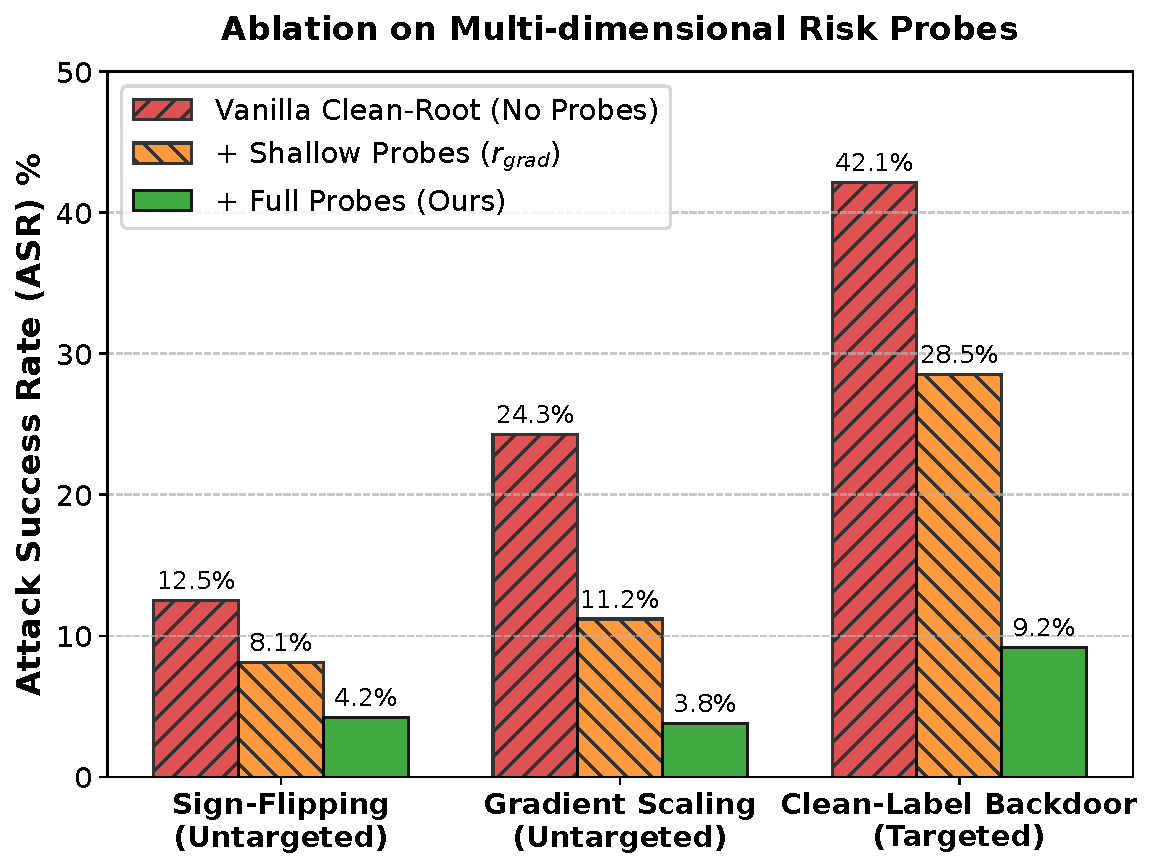
\includegraphics[width=\linewidth]{fig9_ablation_probes.pdf}
        \vspace{-3pt}
        {\scriptsize (a) Multi-dimensional risk-probe ablation.}
    \end{minipage}\hfill
    \begin{minipage}{0.49\textwidth}
        \centering
        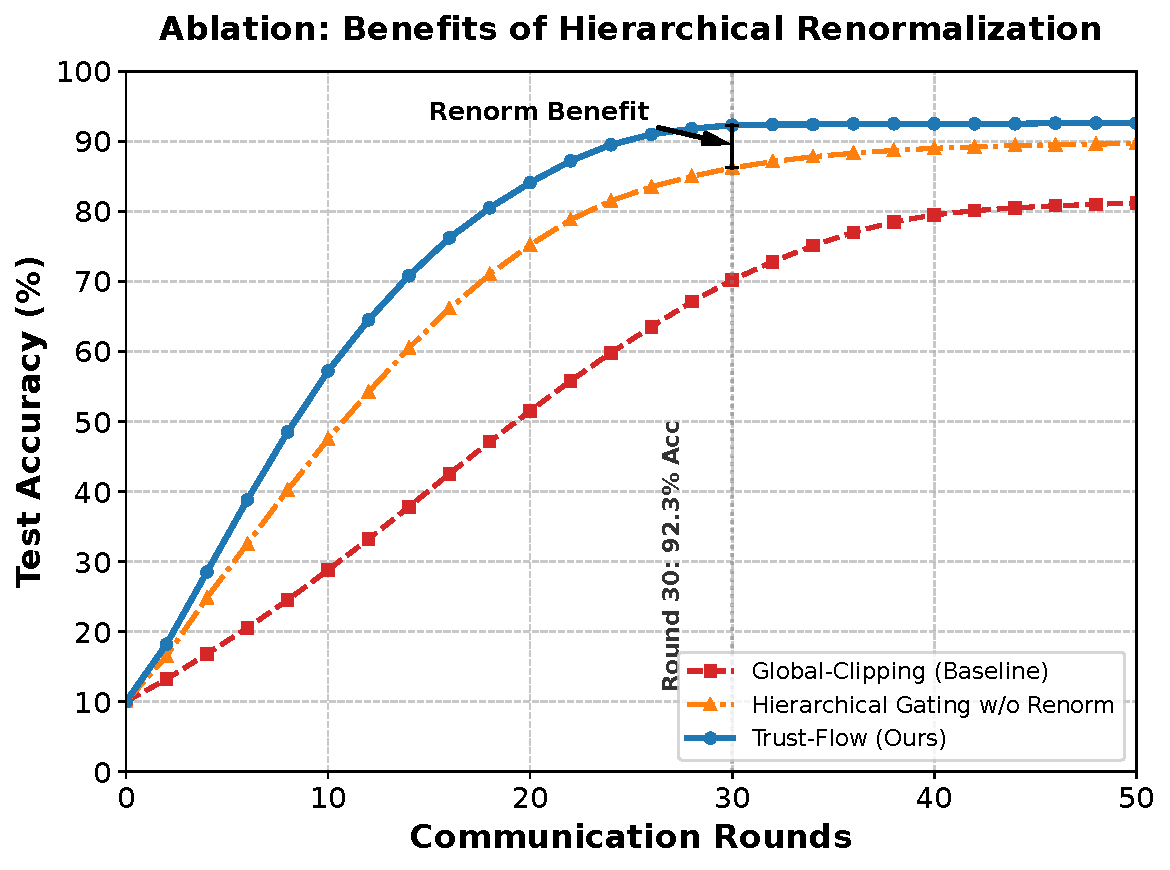
\includegraphics[width=\linewidth]{fig10_ablation_renorm.pdf}
        \vspace{-3pt}
        {\scriptsize (b) Weight re-normalization effect.}
    \end{minipage}
    \caption{Component-level ablation of risk probes and re-normalization.}
    \label{fig:ablation_components}
\end{figure}

\begin{figure}[t]
    \centering
    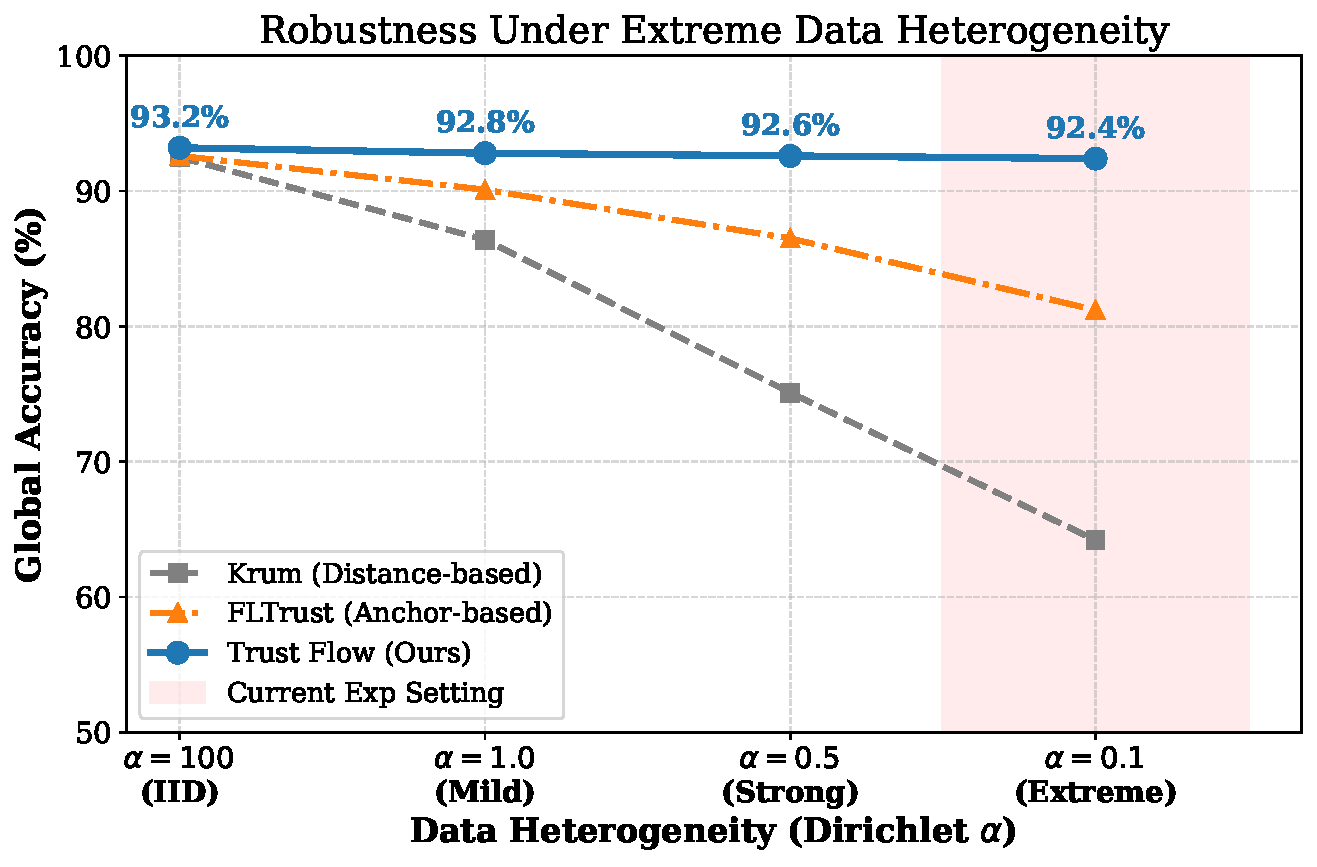
\includegraphics[width=0.76\textwidth]{fig11_alpha_sensitivity.pdf}
    \caption{Robustness stress test under varying data heterogeneity.}
    \label{fig:alpha_sensitivity}
\end{figure}

\section{Discussion and Conclusion}

Trust Flow integrates execution admission, privacy-aware statistical checks, content auditing, temporal reputation, and layer-wise aggregation into a single trust-state pipeline. Its system-level contribution is the ordering and separation of these evidence streams: execution evidence controls admission, privacy-aware checks expose bounded data evidence, current probes control immediate risk, historical utility controls recoverable retention, and layer scores control where an update can contribute. On the two tested Intel and AMD TEE-capable configurations, this separation keeps permanent-ban FPR near zero while maintaining high recall against the tested mixed attacks. The resulting assurance contract makes the boundary explicit: attestation establishes execution eligibility, while cloud-side content and temporal evidence determine update safety.

The evaluated deployment profile is server-assisted vision FL with a small trusted reference partition and an attestation-capable client path. The peer-reference branch extends the same decision sequence to deployments that do not provide a server proxy, while the present measurements focus on the common reference-initialized path. Microarchitectural side channels and vendor-specific enclave resource contention are outside the threat model. The probe design is tailored to vision classification, and the reported overhead is partitioned into server audit, auxiliary secure-path, and device-side attestation components rather than presented as a single end-to-end latency. Cryptographic secure aggregation remains outside the main system boundary because the server must inspect individual evidence. This explicit profile defines where the trust-flow contract applies and provides the basis for extending it to other data modalities and deployment conditions.

\begingroup
\scriptsize
\begin{thebibliography}{99}
    \setlength{\itemsep}{0pt}
    \bibitem{kairouz2021flsurvey} Kairouz, P., McMahan, H.B., Avent, B., et al.: Advances and open problems in federated learning. Foundations and Trends in Machine Learning 14(1--2), 1--210 (2021). \url{https://doi.org/10.1561/2200000083}
    \bibitem{mcmahan2017fedavg} McMahan, B., Moore, E., Ramage, D., Hampson, S., Aguera y Arcas, B.: Communication-efficient learning of deep networks from decentralized data. In: Proceedings of the 20th International Conference on Artificial Intelligence and Statistics, PMLR 54, pp. 1273--1282 (2017). \url{https://proceedings.mlr.press/v54/mcmahan17a.html}
    \bibitem{blanchard2017krum} Blanchard, P., El Mhamdi, E.M., Guerraoui, R., Stainer, J.: Machine learning with adversaries: Byzantine tolerant gradient descent. In: Advances in Neural Information Processing Systems 30 (2017). \href{https://papers.nips.cc/paper/6617-machine-learning-with-adversaries-byzantine-tolerant-gradient-descent}{NeurIPS paper page}
    \bibitem{yin2018byzantine} Yin, D., Chen, Y., Ramchandran, K., Bartlett, P.: Byzantine-robust distributed learning: Towards optimal statistical rates. In: Proceedings of the 35th International Conference on Machine Learning, PMLR 80, pp. 5650--5659 (2018). \url{https://proceedings.mlr.press/v80/yin18a.html}
    \bibitem{cao2021fltrust} Cao, X., Fang, M., Liu, J., Gong, N.Z.: FLTrust: Byzantine-robust federated learning via trust bootstrapping. In: Proceedings 2021 Network and Distributed System Security Symposium (NDSS) (2021). \url{https://doi.org/10.14722/ndss.2021.24434}
    \bibitem{fung2020foolsgold} Fung, C., Yoon, C.J.M., Beschastnikh, I.: The limitations of federated learning in Sybil settings. In: 23rd International Symposium on Research in Attacks, Intrusions and Defenses (RAID 2020), pp. 301--316. USENIX Association (2020). \url{https://www.usenix.org/conference/raid2020/presentation/fung}
    \bibitem{wang2025rasa} Wang, L., Huang, M., Zhang, Z., Li, M., Wang, J., Gai, K.: RaSA: Robust and adaptive secure aggregation for edge-assisted hierarchical federated learning. IEEE Transactions on Information Forensics and Security 20, 4280--4295 (2025). \url{https://doi.org/10.1109/TIFS.2025.3559411}
    \bibitem{fldetector2022} Zhang, Z., Cao, X., Jia, J., Gong, N.Z.: FLDetector: Defending federated learning against model poisoning attacks via detecting malicious clients. In: Proceedings of the 28th ACM SIGKDD Conference on Knowledge Discovery and Data Mining, pp. 2545--2555 (2022). \url{https://doi.org/10.1145/3534678.3539231}
    \bibitem{deepsight2022} Rieger, P., Nguyen, T.D., Miettinen, M., Sadeghi, A.R.: DeepSight: Mitigating backdoor attacks in federated learning through deep model inspection. In: Network and Distributed System Security Symposium (NDSS) (2022). \url{https://doi.org/10.14722/ndss.2022.23156}
    \bibitem{flame2022} Nguyen, T.D., Rieger, P., Chen, H., et al.: FLAME: Taming backdoors in federated learning. In: 31st USENIX Security Symposium, pp. 1415--1432 (2022). \url{https://www.usenix.org/conference/usenixsecurity22/presentation/nguyen}
    \bibitem{flpurifier} Zhang, J., Zhu, C., Sun, X., Ge, C., Chen, B., Susilo, W., Yu, S.: FLPurifier: Backdoor defense in federated learning via decoupled contrastive training. IEEE Transactions on Information Forensics and Security 19, 4752--4766 (2024). \url{https://doi.org/10.1109/TIFS.2024.3384846}
    \bibitem{crowdguard2024} Rieger, P., Krau{\ss}, T., Miettinen, M., Dmitrienko, A., Sadeghi, A.R.: CrowdGuard: Federated backdoor detection in federated learning. In: Network and Distributed System Security Symposium (NDSS) (2024). \url{https://doi.org/10.14722/ndss.2024.23233}
    \bibitem{roseagg} Yang, H., Xi, W., Shen, Y., Wu, C., Zhao, J.: RoseAgg: Robust defense against targeted collusion attacks in federated learning. IEEE Transactions on Information Forensics and Security 19, 2951--2966 (2024). \url{https://doi.org/10.1109/TIFS.2024.3352415}
    \bibitem{shieldfl} Ma, Z., Ma, J., Miao, Y., Li, Y., Deng, R.H.: ShieldFL: Mitigating model poisoning attacks in privacy-preserving federated learning. IEEE Transactions on Information Forensics and Security 17, 1639--1654 (2022). \url{https://doi.org/10.1109/TIFS.2022.3169918}
    \bibitem{r1_tee_integrity} Chen, Y., Luo, F., Li, T., Xiang, T., Liu, Z., Li, J.: A training-integrity privacy-preserving federated learning scheme with trusted execution environment. Information Sciences 522, 69--79 (2020). \url{https://doi.org/10.1016/j.ins.2020.02.037}
    \bibitem{xu2021distributed} Xu, T., Zhu, K., Andrzejak, A., Zhang, L.: Distributed learning in trusted execution environment: A case study of federated learning in SGX. In: 2021 7th IEEE International Conference on Network Intelligence and Digital Content (IC-NIDC), pp. 450--454 (2021). \url{https://doi.org/10.1109/IC-NIDC54101.2021.9660433}
    \bibitem{zhang2025rppfl} Zhang, X., Chen, Z., Chen, G., Feng, X., Shen, Q., Wu, Z.: RPPFL: Robust and privacy-preserving federated learning via trusted execution environments. In: ICASSP 2025 - 2025 IEEE International Conference on Acoustics, Speech and Signal Processing, pp. 1--5 (2025). \url{https://doi.org/10.1109/ICASSP49660.2025.10889398}
    \bibitem{r5_tee_mitigating} Queyrut, S., Schiavoni, V., Felber, P.: Mitigating adversarial attacks in federated learning with trusted execution environments. In: 2023 IEEE 43rd International Conference on Distributed Computing Systems (ICDCS), pp. 626--637 (2023). \url{https://doi.org/10.1109/ICDCS57875.2023.00069}
    \bibitem{lu2025tmt} Lu, Z., Wang, L., Zhang, Z., Huang, M., Wang, J., Li, M.: TMT-FL: Enabling trustworthy model training of federated learning with malicious participants. IEEE Transactions on Dependable and Secure Computing 22(3), 2723--2740 (2025). \url{https://doi.org/10.1109/TDSC.2024.3521377}

    \bibitem{bagdasaryan2020backdoor} Bagdasaryan, E., Veit, A., Hua, Y., Estrin, D., Shmatikov, V.: How To Backdoor Federated Learning. In: Proceedings of the Twenty Third International Conference on Artificial Intelligence and Statistics, PMLR 108, pp. 2938--2948 (2020). \url{https://proceedings.mlr.press/v108/bagdasaryan20a.html}
    \bibitem{wang2019neuralcleanse} Wang, B., Yao, Y., Shan, S., Li, H., Viswanath, B., Zheng, H., Zhao, B.Y.: Neural Cleanse: Identifying and mitigating backdoor attacks in neural networks. In: 2019 IEEE Symposium on Security and Privacy (SP), pp. 707--723 (2019). \url{https://doi.org/10.1109/SP.2019.00031}

\end{thebibliography}
\endgroup

\end{document}
